% Options for packages loaded elsewhere
\PassOptionsToPackage{unicode}{hyperref}
\PassOptionsToPackage{hyphens}{url}
\PassOptionsToPackage{dvipsnames,svgnames,x11names}{xcolor}
%
\documentclass[
]{article}

\usepackage{amsmath,amssymb}
\usepackage{iftex}
\ifPDFTeX
  \usepackage[T1]{fontenc}
  \usepackage[utf8]{inputenc}
  \usepackage{textcomp} % provide euro and other symbols
\else % if luatex or xetex
  \usepackage{unicode-math}
  \defaultfontfeatures{Scale=MatchLowercase}
  \defaultfontfeatures[\rmfamily]{Ligatures=TeX,Scale=1}
\fi
\usepackage{lmodern}
\ifPDFTeX\else  
    % xetex/luatex font selection
\fi
% Use upquote if available, for straight quotes in verbatim environments
\IfFileExists{upquote.sty}{\usepackage{upquote}}{}
\IfFileExists{microtype.sty}{% use microtype if available
  \usepackage[]{microtype}
  \UseMicrotypeSet[protrusion]{basicmath} % disable protrusion for tt fonts
}{}
\makeatletter
\@ifundefined{KOMAClassName}{% if non-KOMA class
  \IfFileExists{parskip.sty}{%
    \usepackage{parskip}
  }{% else
    \setlength{\parindent}{0pt}
    \setlength{\parskip}{6pt plus 2pt minus 1pt}}
}{% if KOMA class
  \KOMAoptions{parskip=half}}
\makeatother
\usepackage{xcolor}
\setlength{\emergencystretch}{3em} % prevent overfull lines
\setcounter{secnumdepth}{-\maxdimen} % remove section numbering
% Make \paragraph and \subparagraph free-standing
\ifx\paragraph\undefined\else
  \let\oldparagraph\paragraph
  \renewcommand{\paragraph}[1]{\oldparagraph{#1}\mbox{}}
\fi
\ifx\subparagraph\undefined\else
  \let\oldsubparagraph\subparagraph
  \renewcommand{\subparagraph}[1]{\oldsubparagraph{#1}\mbox{}}
\fi


\providecommand{\tightlist}{%
  \setlength{\itemsep}{0pt}\setlength{\parskip}{0pt}}\usepackage{longtable,booktabs,array}
\usepackage{calc} % for calculating minipage widths
% Correct order of tables after \paragraph or \subparagraph
\usepackage{etoolbox}
\makeatletter
\patchcmd\longtable{\par}{\if@noskipsec\mbox{}\fi\par}{}{}
\makeatother
% Allow footnotes in longtable head/foot
\IfFileExists{footnotehyper.sty}{\usepackage{footnotehyper}}{\usepackage{footnote}}
\makesavenoteenv{longtable}
\usepackage{graphicx}
\makeatletter
\def\maxwidth{\ifdim\Gin@nat@width>\linewidth\linewidth\else\Gin@nat@width\fi}
\def\maxheight{\ifdim\Gin@nat@height>\textheight\textheight\else\Gin@nat@height\fi}
\makeatother
% Scale images if necessary, so that they will not overflow the page
% margins by default, and it is still possible to overwrite the defaults
% using explicit options in \includegraphics[width, height, ...]{}
\setkeys{Gin}{width=\maxwidth,height=\maxheight,keepaspectratio}
% Set default figure placement to htbp
\makeatletter
\def\fps@figure{htbp}
\makeatother
% definitions for citeproc citations
\NewDocumentCommand\citeproctext{}{}
\NewDocumentCommand\citeproc{mm}{%
  \begingroup\def\citeproctext{#2}\cite{#1}\endgroup}
\makeatletter
 % allow citations to break across lines
 \let\@cite@ofmt\@firstofone
 % avoid brackets around text for \cite:
 \def\@biblabel#1{}
 \def\@cite#1#2{{#1\if@tempswa , #2\fi}}
\makeatother
\newlength{\cslhangindent}
\setlength{\cslhangindent}{1.5em}
\newlength{\csllabelwidth}
\setlength{\csllabelwidth}{3em}
\newenvironment{CSLReferences}[2] % #1 hanging-indent, #2 entry-spacing
 {\begin{list}{}{%
  \setlength{\itemindent}{0pt}
  \setlength{\leftmargin}{0pt}
  \setlength{\parsep}{0pt}
  % turn on hanging indent if param 1 is 1
  \ifodd #1
   \setlength{\leftmargin}{\cslhangindent}
   \setlength{\itemindent}{-1\cslhangindent}
  \fi
  % set entry spacing
  \setlength{\itemsep}{#2\baselineskip}}}
 {\end{list}}
\usepackage{calc}
\newcommand{\CSLBlock}[1]{\hfill\break\parbox[t]{\linewidth}{\strut\ignorespaces#1\strut}}
\newcommand{\CSLLeftMargin}[1]{\parbox[t]{\csllabelwidth}{\strut#1\strut}}
\newcommand{\CSLRightInline}[1]{\parbox[t]{\linewidth - \csllabelwidth}{\strut#1\strut}}
\newcommand{\CSLIndent}[1]{\hspace{\cslhangindent}#1}

\usepackage[noblocks]{authblk}
\renewcommand*{\Authsep}{, }
\renewcommand*{\Authand}{, }
\renewcommand*{\Authands}{, }
\renewcommand\Affilfont{\small}
\makeatletter
\@ifpackageloaded{caption}{}{\usepackage{caption}}
\AtBeginDocument{%
\ifdefined\contentsname
  \renewcommand*\contentsname{Table of contents}
\else
  \newcommand\contentsname{Table of contents}
\fi
\ifdefined\listfigurename
  \renewcommand*\listfigurename{List of Figures}
\else
  \newcommand\listfigurename{List of Figures}
\fi
\ifdefined\listtablename
  \renewcommand*\listtablename{List of Tables}
\else
  \newcommand\listtablename{List of Tables}
\fi
\ifdefined\figurename
  \renewcommand*\figurename{Figure}
\else
  \newcommand\figurename{Figure}
\fi
\ifdefined\tablename
  \renewcommand*\tablename{Table}
\else
  \newcommand\tablename{Table}
\fi
}
\@ifpackageloaded{float}{}{\usepackage{float}}
\floatstyle{ruled}
\@ifundefined{c@chapter}{\newfloat{codelisting}{h}{lop}}{\newfloat{codelisting}{h}{lop}[chapter]}
\floatname{codelisting}{Listing}
\newcommand*\listoflistings{\listof{codelisting}{List of Listings}}
\makeatother
\makeatletter
\makeatother
\makeatletter
\@ifpackageloaded{caption}{}{\usepackage{caption}}
\@ifpackageloaded{subcaption}{}{\usepackage{subcaption}}
\makeatother
\ifLuaTeX
  \usepackage{selnolig}  % disable illegal ligatures
\fi
\usepackage{bookmark}

\IfFileExists{xurl.sty}{\usepackage{xurl}}{} % add URL line breaks if available
\urlstyle{same} % disable monospaced font for URLs
\hypersetup{
  pdftitle={Advancing spatially explicit fisheries management with age-structured species distribution models},
  pdfauthor={Eric Ward; Nick Tolimieri},
  colorlinks=true,
  linkcolor={blue},
  filecolor={Maroon},
  citecolor={Blue},
  urlcolor={Blue},
  pdfcreator={LaTeX via pandoc}}

  \title{Advancing spatially explicit fisheries management with
age-structured species distribution models}
  
    
    \author{Eric Ward}
    \author{Nick Tolimieri}
    \affil{%
          Conservation Biology Division, Northwest Fisheries Science
          Center, National Marine Fisheries Service, National
          Oceanographic and Atmospheric Administration, 2725 Montlake
          Blvd E, Seattle WA 98112
        }
      
  \date{}
\begin{document}
\maketitle

\subsection{\texorpdfstring{\emph{Abstract}}{Abstract}}\label{abstract}

Species distribution models (SDMs) are widely used in fisheries and
ecology, providing insights into species' spatial distributions. While
many SDMs incorporate external information, such as environmental or
habitat features, the majority overlook age-specific information,
despite the known influence of age structure on fish distribution and
abundance. Including age information may be particularly valuable for
species exhibiting age-related spatial patterns driven by ontogenetic
shifts, recruitment dynamics, and selective fishing pressures. Here, we
develop an age-structured SDM framework using data from the west coast
of the USA, and concentrate on two species with distinct life histories:
North Pacific hake (\emph{Merluccius productus}) and sablefish
(\emph{Anoplopoma fimbria}). Our framework uses spatiotemporal models to
predict age-specific distributions. We validate our approach using the
recursive nature of age data to forecast the spatial distribution of
fish by age class across survey locations in subsequent years; these
results highlight that forecast models have predictive skill (more so
for sablefish than hake) and the predictive ability is highest for older
age classes. Output from our models can be used to predict the spatial
age composition, which may be particularly useful for identifying large
cohorts (hake from 2008, 2010, 2014 and 2016 cohorts; sablefish from
2008, 2010, 2016, and 2021 cohorts). Using predictions of age-1
sablefish as an example, we also demonstrate how our models may be used
to forecast future bycatch risk in space, helping increase the
efficiency of fisheries. Our framework is applicable to a wide range of
survey types and platforms around the world, and supports the
development of spatially explicit management strategies and optimal
allocation of fishing effort.

\subsection{Introduction}\label{introduction}

Species distribution models (SDMs) are widely used in marine ecology to
understand and predict the spatial distribution of species based on
environmental and demographic variables (Melo-Merino et al., 2020).
These models have informed management decisions for conservation and
resource allocation, especially in the face of changing environmental
conditions and human impacts, such as fishing pressure (Elith \&
Leathwick, 2009; Guisan \& Thuiller, 2005). Recent advances in SDM
applications in the marine environment have incorporated external
drivers such as temperature (Fredston et al., 2021) and habitat features
(Laman et al., 2018; Phillips et al., 2017). A second use of these
models has been to predict temporal trends in species biomass from
spatiotemporal fisheries independent survey data (Thorson et al., 2015).
Trends estimated from SDMs may be included in integrated population
models (stock assessments) for commercially fished species, or used to
identify risks to populations of conservation concern. Recent
developments in these models have included depth (Johnson et al., 2019)
and habitat variables (Cao et al., 2017) to improve trend estimation.

While many SDMs around the world have included variables such as
temperature, depth, or habitat, they have generally overlooked age
structure, and instead modeled either species occurrences or densities
across all age or size classes. Omitting information on age or size may
be partially dependent on data availability (ageing fish generally
requires sampling otoliths, which increases monetary costs of sampling
programs), but may also be driven by the modeling choices of analysts.
Much of the previous research around the world has demonstrated that age
structure is a fundamental characteristic of fish populations,
influencing spatial distribution and abundance due to mechanisms like
ontogenetic shifts, recruitment variability, and selective fishing
pressures (Rijnsdorp et al., 2018). Recent work has also highlighted
that age-based SDMs can improve understanding of environmental drivers
on commercially valuable populations (Ono et al., 2024). Ignoring
age-specific information in SDMs may lead to incomplete or inaccurate
predictions, especially for species with strong age-related spatial
gradients.

Incorporating age structure into SDMs may provide more accurate
predictions by capturing spatial and temporal variability related to
life history traits, age-specific habitat preferences, and population
dynamics. Fish often exhibit ontogenetic shifts, where younger
individuals occupy different habitats than adults due to factors like
predator avoidance, habitat preferences, and diet changes (Ciannelli et
al., 2004; Werner \& Gilliam, 1984). These shifts can create
age-specific distributions across habitats, particularly for species
that undergo distinct life history phases. Additionally, spatiallly
variable recruitment pulses and age-related migration patterns can
influence the spatial distribution of younger versus older fish. Fishing
selectivity often further accentuates these patterns by
disproportionately removing larger, older fish, which alters the
population structure and potentially shifts spatial distributions
(Hilborn \& Walters, 1992; Methot \& Wetzel, 2013). By incorporating
age, SDMs could better predict these dynamics and improve our
understanding of species-environment relationships.

Because of the recursive nature of population dynamics, e.g.~numbers at
age \emph{a} at time \emph{t} can be used to predict numbers at age
\emph{a}+1 at time \emph{t}+1, age-structured SDMs with predictive skill
also provide a tool for forward prediction, with considerable
implications for marine resource management. Reliable predictions of
species distributions can help managers anticipate and mitigate issues
such as bycatch risk by identifying regions with high densities of
specific age cohorts (Lewison et al., 2004). Forecasting the spatial
distribution of certain age classes can inform spatially explicit
management strategies and help optimize fishing effort to target
sustainable cohorts. For example, knowing the expected future locations
of specific age classes could aid in creating time-area closures that
protect vulnerable life stages or ensure harvests focus on more
resilient portions of the population. However, building robust
age-structured SDMs requires high-quality, long-term datasets with
consistent sampling methods across both age and space to ensure the
validity of these predictions.

Around the world, age and life history information is routinely
collected by a number of sampling platforms, including from fisheries
and fisheries independent surveys. While fisheries dependent data may be
used to inform age structured models, sampling from fisheries
independent surveys is typically more consistent in space and time. The
primary objective of our paper is to explore the utility of developing
age - structured SDMs from fisheries independent data. Focusing on two
species with contrasting life history characteristics in the North
Pacific, the semi-pelagic North Pacific hake (\emph{Merluccius
productus}) and longer lived benthic sablefish (\emph{Anoplopoma
fimbria}), we first develop a flexible framework for modeling numbers at
age. Second, we evaluate the ability of this framework to offer
predictive skill in future forecasts, and quantify how the predictive
relationship changes as a function of age. Finally, we demonstrate how
model output may be used to examine changing species compositions
through time, make maps of potential bycatch hotspots, and identify
areas with higher concentrations of mature fish as potential targets of
fishing effort.

\subsection{Methods}\label{methods}

\subsubsection{Data}\label{data}

On the west coast of the USA, the West Coast Groundfish Bottom Trawl
Survey (WCGBTS) has been an annual survey conduced from 2003 - present.
The WCGBTS is designed to estimate the abundance, size, and age
composition of groundfish species important to commercial and
recreational fisheries found in near-bottom habitats on the west coast
of the USA (Keller et al., 2017). The survey effort is concentrated in
summer months and has been conducted annually since 2003 (here we use
the data through 2018; data are publicly available at
https://www.nwfsc.noaa.gov/data). Importantly, the random stratified
sampling design, spatial and seasonal coverage, effort, and gears have
remained relatively constant within the period we analyze. Like many
other surveys around the world, no WCGBTS survey occurred in 2020
because of the Covid-19 pandemic. Though the WCGBTS survey samples
hundreds of species, we concentrated our analysis on two of the well
sampled species from the WCGBTS, North Pacific hake and sablefish.
{[}more on biological gradients{]} While otoliths are sampled
continuously during the WCGBTS survey for a broad range of species,
otoliths are generally aged when species are being prioritized for stock
assessment by the Pacific Fishery Management Council (PFMC); full
assessments between species may occur irregularly and be sporadically
updated every 5 -- 10 years. Hake and sablefish represent exceptions, as
the hake stock is assessed annually by co-managers from the USA and
Canada (Grandin et al., 2024) and sablefish is frequently assessed
because of its high commercial value. For our analysis, we used hake
collected 2007 -- 2019 (mean 650.7 individuals sampled per year) and
sablefish collected 2003 -- 2023 (mean 1314.4 individuals sampled per
year).

\subsubsection{Spatial age models}\label{spatial-age-models}

For each species, we filtered by sex to focus on females and truncated
ages to focus on those with the highest data availability; for hake this
included ages 1 -- 5, and for sablefish ages 0 -- 9 (data from these
ages represented 54\% and 75\% of the total aged fish, respectively).
For each species - age combination, we constructed a unique
spatiotemporal model fit to all years except the last available year for
each species. We adopted this approach instead of modeling ages
simultaneously (Ono et al., 2024), because this framework allows greater
flexibility (e.g.~unique autocorrelation and spatial variance parameters
by age). Individual fish were aggregated at the haul level, allowing us
to model counts at age with a Poisson distribution. We constructed a
spatiotemporal model as an extension of Generalized Linear Mixed Models
(GLMMs) such that the prediction in location \(s\) and time \(t\) can be
written as

\[
\begin{aligned}
log \left( u_{\boldsymbol{s},t} \right) &= \boldsymbol{\beta_{t}} + \omega_{\boldsymbol{s}} + \delta_{\boldsymbol{s},t}
\end{aligned}
\]

where \(\boldsymbol{\beta_{t}}\) represent time - varying intercepts
modeled as a random walk
\(\boldsymbol{\beta_{t}} \sim N \left( \boldsymbol{\beta_{t-1}}, \sigma_\beta \right)\),
the spatial field
\(\boldsymbol{\omega_{s}} \sim \operatorname{MVNormal} \left( \boldsymbol{0}, \boldsymbol{\Sigma}_\omega \right)\)
and the spatiotemporal fields \(\delta_{\boldsymbol{s},t}\) are modeled
as an AR(1) process
\(\boldsymbol{\delta}_{t} = \rho \boldsymbol{\delta}_{t-1} + \sqrt{1 - \rho^2} \boldsymbol{\epsilon_{t}}\),
where
\(\boldsymbol{\epsilon_{t}} \sim \operatorname{MVNormal} \left(\boldsymbol{0}, \boldsymbol{\Sigma}_{\epsilon} \right)\)

Spatial and spatiotemporal random fields were constructed as Gaussian
Markov random fields (GMRFs) using the stochastic partial differential
equation approach (SPDE) (Lindgren et al., 2011; Lindgren \& Rue, 2015).
The SPDE method models the spatial correlation between points as a
Matérn covariance function with smoothness parameter \(\nu = 1\).
Spatial meshes for all ages and species were constructed with a cutoff
distance of 50km (this distance controls the spacing of mesh vertices).
Parameter estimation was done using the sdmTMB software package
(Anderson et al., 2024) with R 4.3.1 (R Core Team, 2024). The sdmTMB
package relies on Template Model Builder (TMB)(Kristensen et al., 2016)
to quickly and efficiently maximize the marginal log likelihood using
auto-differentiation and the Laplace approximation to integrate out
random effects. Models were evaluated for convergence (positive-definite
Hessian matrix, and a maximum absolute log likelihood gradient
\textless{} 0.001) and residuals diagnostics were evaluated with the
DHARMa package (Hartig, 2022). Code and data to replicate our analysis
is publicly available on Github,
\url{https://github.com/ericward-noaa/spatial-age-models}.

\subsubsection{Validating future predictive
ability}\label{validating-future-predictive-ability}

As a first validation, we leveraged the natural recursive element of our
data to quantify the ability of our models to predict the future
distribution by age. For each of the species - age models constructed
above, we made predictions to the survey locations in the following year
(e.g.~age 3 hake in years 2007 -- 2018 was used to predict the
distribution of age 4 hake in 2008 -- 2019). We related the predictions
\(\hat{u}_{\boldsymbol{s},t}\) to observations by multiplying
predictions by the total number of fish sampled for ageing,
\(\hat{n}_{s,t} = N_{s,t} \cdot \hat{u}_{\boldsymbol{s},t}\). We
quantified the relationship between predictions and observations by
fitting a simple Poisson GLM, where counts of fish of age \(a+1\) in
year \(t+1\) were treated as the response and
\(log(\lambda_{s,t}) = \beta_{0} + \beta_{1} \cdot log \left( \hat{n}_{s,t} \right)\).
The exponentiated slope parameter \(exp(\beta_{1})\) represents a change
in expected counts that would be expected from a 1-unit change in
\(log(\hat{n}_{s,t})\). As a diagnostic check and to understand whether
there was potential temporal patterns in the response, we fit a second
model as a GLMM with R package glmmTMB (Brooks et al., 2017); this
second model was identical to our Poisson GLM with random effects in
\(\beta_{0}\) and \(\beta_{1}\), where year was used as the grouping
variable.

\subsubsection{Using predictions to quantify bycatch
risk}\label{using-predictions-to-quantify-bycatch-risk}

To illustrate potential benefits to fisheries management, we used output
from our models to generate spatiotemporal predictions of age-1
sablefish (from age-0 sablefish the year prior). Sablefish are part of
the DTS complex, which includes Dover sole \emph{Microstomus pacificus},
shortspine \emph{Sebastomus alascanus,} longspine thornyheads \emph{S.
altivelis}, and sablefish. This complex forms and important fishery on
the West Cast, and by-catch of sablefish can impact quotas for the other
three species, as well as the at-sea hake fishery. For exmaple, in 2017,
the at-sea hake fishery had 50 mt of sablefish quota set aside in the
area north of 36 °N, but the fleet caught more than 3x as much, promting
in-season warnings to alter fishing behavior.

Gridded predictions from the Poisson GLM represent the expected number
of fish per unit of effort in each location. To turn these into a
potentially more useful measure of risk, we calculate the predicted
total age-1 sablefish catch per unit of effort (CPUE) within a given
radius of major fishing ports on the US west coast. For consistency with
previous work , we used a radius of 282 km (Leising et al., 2024). These
predictions of port-level CPUE were then summarized as annual time
series (1-step ahead forecasts).

\subsection{Results}\label{results}

One useful output from our spatiotemporal models is the estimated field
spatial f, \(\omega_s\), representing the average spatial distribution
across years. Results from our model of North Pacific hake show a
concentration of age-1 hake near the coast, and more of latitudinal
north - south break for 2 - 3 year old hake (with higher occurrences in
the South, Fig.~\ref{fig-hake-spatial-anomaly}). As expected, age 4 hake
appear to have a northern distribution, though the gradient is less
clear than for ages 2 - 3. For sablefish, our models estimate a
concentration of age 0 - 2 sablefish in shallow water, with a deeper
distribution by age 3 (Fig.~\ref{fig-sablefish-spatial-anomaly}).
Latitudinally, there are several areas in central Oregon that appear to
have consistently lower occurrences than average for older age classes
(Fig.~\ref{fig-sablefish-spatial-anomaly}).

Estimates of age composition by year may be useful in tracking the
distribution of cohorts through time, as well as examining variability
in distributions of particular age classes over time. For example, for
both hake (Figs.~\ref{fig-hake-spatial-composition} \&
\ref{fig-hake-spatial-composition-all}) and sablefish
(Figs.~\ref{fig-sablefish-spatial-composition} \&
\ref{fig-sablefish-spatial-composition-all}), distinct patches of high
age-0 abundance tended to disperse as the fish aged such that spatial
distributions for older age-classes were less distinct. Additionally,
results from our models can be used to project the spatial distributions
of strong hake cohorts (2008, 2010, 2014, 2016;
Fig.~\ref{fig-hake-spatial-composition}) and strong sablefish cohorts
(2008, 2010, 2016, 2021, Fig.~\ref{fig-sablefish-spatial-composition}).
These predictions are also useful in revealing subtle differences
between strong cohort years. For example, the 2014 cohort of Pacific
hake had a larger fraction of age-1 individuals distributed in the
northern part of the domain (along the coast of Washington state), while
other cohorts had hotspots in the center and southern portion of the
domain. Similarly for sablefish, the 2016 cohort was concentrated in the
north (age-1 individuals in 2011), versus other cohorts that had a more
coastwide distribution. In fact, age-1 fish were uncommon south of
approximately Cape Mendocino (40 °N) from 2015 - 2020
(Figure~\ref{fig-sablefish-spatial-composition-all}), concurrent with
`the Blob' and other marine heatwaves.

When comparing the spatial and spatiotemporal parameters across ages and
species, we find that for most ages, there is a decrease in the
estimated spatial and spatiotemporal variances as well as a decrease in
the spatial range with increasing age
(Fig.~\ref{fig-spatial-parameters}). Spatial and spatiotemporal
variances control the magnitude of the peaks and valleys in estimated
latent fields, meaning that spatial fields estimated for older fish are
less variable. Similarly, the spatial range determines the distance at
which locations are functionally independent (for the Matern, \(\rho\)
\textasciitilde{} 0.13). The decline in range with age implies that
spatial distributions also become more concentrated as a function of age
(Fig.~\ref{fig-spatial-parameters}).

Our 1-step ahead validation analyses indicate that there is a stronger
association between older ages compared to younger ages, and this effect
is strongest for sablefish (Fig.~\ref{fig-glm-coefficients}). When
comparing our initial Poisson GLM to a more complicated GLMM with random
year effects in the intercept and slope, we found little support for
shared correlations across age classes of a given species. Shared
correlations would indicate for example that age-2 and age-3 sablefish
may be more or less predictable in certain years (indicating that
information about one age class may be useful in predicting another).
With the exception of a strong positive correlation between age-0 and
age-1 sablefish, most correlations between age classes were smaller than
0.3 in magnitude (Figure~\ref{fig-glm-coefficients-time}).

Our forecasts of age-1 sablefish CPUE illustrates the variability of
potential bycatch risk in space and time. In most years for example,
age-1 CPUE is lowest in ports in the state of California (Eureka, Fort
Bragg, Morro Bay) and highest in several ports in the state of Oregon
(Astoria, Coos Bay, Fig.~\ref{fig-bycatch-risk}). These results also
illustrate the high temporal variability in age-1 CPUE, with peaks
occuring in 2009, 2014, 2017, and 2021, Figure~\ref{fig-bycatch-risk}).
During peak years, there is also variability among ports -- forecasts of
age-1 CPUE were similar for Astoria and Coos Bay in 2021 for instance,
but the potential bycatch risk near Astoria was higher in 2017
(Fig.~\ref{fig-bycatch-risk}).

\subsection{Discussion}\label{discussion}

In this study, we developed an age-structured species distribution
modeling (SDM) framework to explore spatial age composition and predict
age-specific distributions of two commercially important fish species
with different life history characteristics: North Pacific hake and
sablefish. Our approach integrates spatiotemporal dynamics, age
structure, and forward-predictive capabilities, providing a useful tool
for fisheries management. By examining age-specific patterns in spatial
distributions and validating predictive skill, we highlight the
potential utility of incorporating age structure into SDMs for advancing
spatially explicit fisheries management.

\paragraph{\texorpdfstring{\emph{Age-Structured Spatial
Patterns}}{Age-Structured Spatial Patterns}}\label{age-structured-spatial-patterns}

Results from our age-structured spatial models underscore the importance
of accounting for age in SDMs. The spatial patterns observed for both
hake and sablefish were consistent with their distinct life histories,
supporting the idea that ontogenetic shifts significantly influence fish
distributions. Younger age classes of hake and sablefish exhibited
broader distributions generally in shallower areas, while older
individuals were more concentrated offshore (sablefish in deeper waters,
hake in more northern regions). The deeper distribution of older
sablefish reflects their preference for benthic habitats and an
ontogenetic shift to deeper waters, while the observed north-south
gradient in older hake aligns with known migratory behaviors influenced
by spawning and feeding grounds (Agostini et al., 2006).

\paragraph{\texorpdfstring{\emph{Predictive skill and cohort
tracking}}{Predictive skill and cohort tracking}}\label{predictive-skill-and-cohort-tracking}

Our validation analyses revealed that the predictive skill of our
framework increases with age, particularly for sablefish. This result is
intuitive given that older age classes generally exhibit more stable
spatial patterns due to reduced recruitment variability and more
predictable habitat preferences. In contrast, the lower predictive skill
for younger age classes reflects their higher spatiotemporal
variability, likely driven by recruitment pulses and early-life survival
dynamics. Tracking cohorts through time using our framework proved
effective in identifying strong year classes
(Figs.~\ref{fig-hake-spatial-composition} \&
\ref{fig-hake-spatial-composition}). Identifying these cohorts may be
useful to stock assessment and management -- for instance, understanding
the spatial distribution of strong cohorts could be used to inform
spatial harvest allocation. Additionally, the ability to project spatial
age composition provides a tool for assessing how environmental changes,
such as ocean warming or habitat shifts, may impact the distribution of
key cohorts over time.

\paragraph{\texorpdfstring{\emph{Managing bycatch
risk}}{Managing bycatch risk}}\label{managing-bycatch-risk}

Our case study using age-1 sablefish demonstrates the practical utility
of our modeling for mitigating bycatch risk. Forecasts of CPUE for age-1
sablefish revealed significant temporal and spatial variability, with
higher bycatch risk near Oregon ports in certain years. Importantly,
these forecasts could be provided to industry partners and fisheries
managers 6 -- 12 months before fishing occurs. Such information could
help fishers avoid areas associated with high bycatch risk, or be used
to adjust the spatial distribution of quota in certain years. The
observed peaks in age-1 sablefish CPUE during certain years suggest the
influence of recruitment pulses, which are thought to be tied to
environmental drivers (Tolimieri et al., 2018; Tolimieri \& Haltuch,
2023). Future efforts could also incorporating environmental covariates
to enhance its predictive accuracy and further support climate-resilient
fisheries management.

\paragraph{Need for reliable age data}\label{need-for-reliable-age-data}

Perhaps the biggest challenge in implementing our modeling framework in
the future is that these models depend on reliable age data being
collected. While the WCGBTS provides a robust dataset, gaps in sampling
(e.g., the absence of a 2020 survey due to the COVID-19 pandemic) and
variability in otolith aging efforts over time could introduce
uncertainty. The costs of ship-based surveys, such as the WCGBTS survey,
have increased around the world, and numerous efforts are being
implemented to make these programs more efficient (ICES, 2020). While
age samples are more expensive to collect than length information, there
is value from the increased precision associated with age data.

\paragraph{Future directions}\label{future-directions}

Our age-structured SDM framework represents a significant advance in
spatial modeling, offering novel insights into the dynamics of fish
populations and their age-specific distributions. From a management
perspective, age-structured SDMs offer a powerful tool for addressing
critical challenges, including bycatch mitigation, spatial planning, and
sustainable harvesting. By providing high-resolution predictions of
spatial age composition, these models enable managers to align fishing
effort with ecological and economic goals, ensuring the long-term
sustainability of marine resources. Future research could extend this
framework by incorporating environmental covariates, such as temperature
or oxygen, to account for dynamic habitat preferences, or fisheries
removals to account for local depletion (Ono et al., 2016).
Additionally, exploring the potential for multi-species models could
provide insights into ecosystem-level interactions and their influence
on spatial distributions.

\subsubsection{Acknowledgments}\label{acknowledgments}

We thank Owen Liu and Chris Jordan for constructive comments on the
manuscript.

\break
\clearpage

\subsection{References}\label{references}

\phantomsection\label{refs}
\begin{CSLReferences}{1}{0}
\bibitem[\citeproctext]{ref-agostini2006}
Agostini, V. N., Francis, R. C., Hollowed, A. B., Pierce, S. D., Wilson,
C., \& Hendrix, A. N. (2006). {The relationship between Pacific hake
({\emph{Merluccius productus}}) distribution and poleward subsurface
flow in the California Current System}. \emph{Canadian Journal of
Fisheries and Aquatic Sciences}, \emph{63}(12), 2648--2659.
\url{https://doi.org/10.1139/f06-139}

\bibitem[\citeproctext]{ref-Anderson2024}
Anderson, S. C., Ward, E. J., English, P. A., Barnett, L. A. K., \&
Thorson, J. T. (2024). {sdmTMB: An R package for fast, flexible, and
user-friendly generalized linear mixed effects models with spatial and
spatiotemporal random fields}. \emph{bioRxiv}.
\url{https://doi.org/10.1101/2022.03.24.485545}

\bibitem[\citeproctext]{ref-brooks2017}
Brooks, E., M., Kristensen, K., Benthem, A. van, K. J.and Magnusson,
Berg, C. W., Nielsen, A., Skaug, H. J., Mächler, M., \& Bolker, M., B.
(2017). {glmmTMB balances speed and flexibility among packages for
zero-inflated generalized linear mixed modeling}. \emph{The R Journal},
\emph{9}(2), 378. \url{https://doi.org/10.32614/rj-2017-066}

\bibitem[\citeproctext]{ref-cao2017}
Cao, J., Thorson, J. T., Richards, R. A., \& Chen, Y. (2017).
{Spatiotemporal index standardization improves the stock assessment of
northern shrimp in the Gulf of Maine}. \emph{Canadian Journal of
Fisheries and Aquatic Sciences}, \emph{74}(11), 1781--1793.
\url{https://doi.org/10.1139/cjfas-2016-0137}

\bibitem[\citeproctext]{ref-ciannelli2004}
Ciannelli, L., Chan, K.-S., Bailey, K. M., \& Stenseth, N. Chr. (2004).
{Nonadditive effects of the environment on the survival of a large
marine fish population}. \emph{Ecology}, \emph{85}(12), 3418--3427.
\url{https://doi.org/10.1890/03-0755}

\bibitem[\citeproctext]{ref-elith2009}
Elith, J., \& Leathwick, J. R. (2009). {Species distribution models:
Ecological explanation and prediction across space and time}.
\emph{Annual Review of Ecology, Evolution, and Systematics},
\emph{40}(1), 677--697.
\url{https://doi.org/10.1146/annurev.ecolsys.110308.120159}

\bibitem[\citeproctext]{ref-fredston2021}
Fredston, A., Pinsky, M., Selden, R. L., Szuwalski, C., Thorson, J. T.,
Gaines, S. D., \& Halpern, B. S. (2021). {Range edges of North American
marine species are tracking temperature over decades}. \emph{Global
Change Biology}, \emph{27}(13), 3145--3156.
\url{https://doi.org/10.1111/gcb.15614}

\bibitem[\citeproctext]{ref-Grandin2024}
Grandin, C. J., Johnson, K. F., M., E. A., \& M., B. A. (2024).
\emph{{Status of the Pacific Hake (whiting) stock in U.S. and Canadian
waters in 2024. Prepared by the Joint Technical Committee of the U.S.
and Canada Pacific Hake/Whiting Agreement, National Marine Fisheries
Service and Fisheries and Oceans Canada. 246 p.}}

\bibitem[\citeproctext]{ref-guisan2005}
Guisan, A., \& Thuiller, W. (2005). {Predicting species distribution:
offering more than simple habitat models}. \emph{Ecology Letters},
\emph{8}(9), 993--1009.
\url{https://doi.org/10.1111/j.1461-0248.2005.00792.x}

\bibitem[\citeproctext]{ref-dharma2022}
Hartig, F. (2022). \emph{{DHARMa: Residual diagnostics for hierarchical
(multi-level / mixed) regression models}}.
\url{https://CRAN.R-project.org/package=DHARMa}

\bibitem[\citeproctext]{ref-hilborn1992}
Hilborn, R., \& Walters, C. J. (1992). \emph{{Quantitative fisheries
stock assessment}}. Springer US.
\url{https://doi.org/10.1007/978-1-4615-3598-0}

\bibitem[\citeproctext]{ref-ices2020}
ICES. (2020). {Workshop on unavoidable survey effort reduction
(WKUSER)}. \emph{ICES}. \url{https://doi.org/10.17895/ICES.PUB.7453}

\bibitem[\citeproctext]{ref-johnson2019}
Johnson, K. F., Thorson, J. T., \& Punt, A. E. (2019). {Investigating
the value of including depth during spatiotemporal index
standardization}. \emph{Fisheries Research}, \emph{216}, 126--137.
\url{https://doi.org/10.1016/j.fishres.2019.04.004}

\bibitem[\citeproctext]{ref-keller2017}
Keller, A. A., Wallace, J. R., \& Methot, R. D. (2017). \emph{{The
Northwest Fisheries Science Center's West coast groundfish bottom trawl
survey: History design, and description}}. NOAA, U.S. Department of
Commerce. \url{https://doi.org/10.7289/V5/TM-NWFSC-136}

\bibitem[\citeproctext]{ref-kristensen2016}
Kristensen, K., Nielsen, A., Berg, C. W., Skaug, H., \& Bell, B. M.
(2016). {TMB: Automatic differentiation and laplace approximation}.
\emph{Journal of Statistical Software}, \emph{70}(5).
\url{https://doi.org/10.18637/jss.v070.i05}

\bibitem[\citeproctext]{ref-laman2018}
Laman, E. A., Rooper, C. N., Turner, K., Rooney, S., Cooper, D. W., \&
Zimmermann, M. (2018). {Using species distribution models to describe
essential fish habitat in Alaska}. \emph{Canadian Journal of Fisheries
and Aquatic Sciences}, \emph{75}(8), 1230--1255.
\url{https://doi.org/10.1139/cjfas-2017-0181}

\bibitem[\citeproctext]{ref-leising2024cciea}
Leising, A., M., H., N., T., G., W., \& A., H. (2024).

\bibitem[\citeproctext]{ref-lewison2004}
Lewison, R. L., Freeman, S. A., \& Crowder, L. B. (2004). {Quantifying
the effects of fisheries on threatened species: the impact of pelagic
longlines on loggerhead and leatherback sea turtles}. \emph{Ecology
Letters}, \emph{7}(3), 221--231.
\url{https://doi.org/10.1111/j.1461-0248.2004.00573.x}

\bibitem[\citeproctext]{ref-lindgren2015}
Lindgren, F., \& Rue, H. (2015). {Bayesian spatial modelling
with{\emph{R}}-{\textbf{INLA}}}. \emph{Journal of Statistical Software},
\emph{63}(19). \url{https://doi.org/10.18637/jss.v063.i19}

\bibitem[\citeproctext]{ref-lindgren2011}
Lindgren, F., Rue, H., \& Lindström, J. (2011). {An explicit link
between Gaussian fields and Gaussian Markov Random Fields: The
dtochastic partial fifferential rquation spproach}. \emph{Journal of the
Royal Statistical Society Series B: Statistical Methodology},
\emph{73}(4), 423--498.
\url{https://doi.org/10.1111/j.1467-9868.2011.00777.x}

\bibitem[\citeproctext]{ref-melo-merino2020}
Melo-Merino, S. M., Reyes-Bonilla, H., \& Lira-Noriega, A. (2020).
{Ecological niche models and species distribution models in marine
environments: A literature review and spatial analysis of evidence}.
\emph{Ecological Modelling}, \emph{415}, 108837.
\url{https://doi.org/10.1016/j.ecolmodel.2019.108837}

\bibitem[\citeproctext]{ref-methot2013}
Methot, R. D., \& Wetzel, C. R. (2013). {Stock synthesis: A biological
and statistical framework for fish stock assessment and fishery
management}. \emph{Fisheries Research}, \emph{142}, 86--99.
\url{https://doi.org/10.1016/j.fishres.2012.10.012}

\bibitem[\citeproctext]{ref-ono2024}
Ono, K., Katara, I., Eliasen, S. K., Broms, C., Campbell, A., dos Santos
Schmidt, T. C., Egan, A., Hølleland, S. N., Jacobsen, J. A., Jansen, T.,
Mackinson, S., Mousing, E. A., Nash, R. D. M., Nikolioudakis, N.,
Nnanatu, C., Nøttestad, L., Singh, W., Slotte, A., Wieland, K., \&
Olafsdottir, A. H. (2024). {Effect of environmental drivers on the
spatiotemporal distribution of mackerel at age in the Nordic Seas during
2010{-}20}. \emph{ICES Journal of Marine Science}, \emph{81}(7),
1282--1294. \url{https://doi.org/10.1093/icesjms/fsae087}

\bibitem[\citeproctext]{ref-ono2016space}
Ono, K., Shelton, A. O., Ward, E. J., Thorson, J. T., Feist, B. E., \&
Hilborn, R. (2016). {Space-time investigation of the effects of fishing
on fish populations}. \emph{Ecological Applications}, \emph{26}(2),
392--406.

\bibitem[\citeproctext]{ref-phillips2017}
Phillips, N. D., Reid, N., Thys, T., Harrod, C., Payne, N. L., Morgan,
C. A., White, H. J., Porter, S., \& Houghton, J. D. R. (2017). {Applying
species distribution modelling to a data poor, pelagic fish complex: the
ocean sunfishes}. \emph{Journal of Biogeography}, \emph{44}(10),
2176--2187. \url{https://doi.org/10.1111/jbi.13033}

\bibitem[\citeproctext]{ref-rcore2024}
R Core Team. (2024). \emph{{R: A language and environment for
statistical computing}}. R Foundation for Statistical Computing.
\url{https://www.R-project.org/}

\bibitem[\citeproctext]{ref-rijnsdorp2018}
Rijnsdorp, A. D., Bolam, S. G., Garcia, C., Hiddink, J. G., Hintzen, N.
T., Denderen, P. D. van, \& Kooten, T. van. (2018). {Estimating
sensitivity of seabed habitats to disturbance by bottom trawling based
on the longevity of benthic fauna}. \emph{Ecological Applications},
\emph{28}(5), 1302--1312. \url{https://doi.org/10.1002/eap.1731}

\bibitem[\citeproctext]{ref-thorson2015}
Thorson, J. T., Shelton, A. O., Ward, E. J., \& Skaug, H. J. (2015).
{Geostatistical delta-generalized linear mixed models improve precision
for estimated abundance indices for West Coast groundfishes}. \emph{ICES
Journal of Marine Science}, \emph{72}(5), 1297--1310.
\url{https://doi.org/10.1093/icesjms/fsu243}

\bibitem[\citeproctext]{ref-tolimieri2023sea}
Tolimieri, N., \& Haltuch, M. (2023). {Sea-level index of recruitment
variability improves assessment model performance for sablefish
/textit{Anoplopoma fimbria}}. \emph{Canadian Journal of Fisheries and
Aquatic Sciences}, \emph{80}(6), 1006--1016.

\bibitem[\citeproctext]{ref-tolimieri2018}
Tolimieri, N., Haltuch, M. A., Lee, Q., Jacox, M. G., \& Bograd, S. J.
(2018). {Oceanographic drivers of sablefish recruitment in the
California Current}. \emph{Fisheries Oceanography}, \emph{27}(5),
458--474. \url{https://doi.org/10.1111/fog.12266}

\bibitem[\citeproctext]{ref-werner1984}
Werner, E. E., \& Gilliam, J. F. (1984). {The ontogenetic niche and
species interactions in size-structured populations}. \emph{Annual
Review of Ecology and Systematics}, \emph{15}(1), 393--425.
\url{https://doi.org/10.1146/annurev.es.15.110184.002141}

\end{CSLReferences}

\break
\clearpage

\subsection{Figures}\label{figures}

\begin{figure}

\centering{

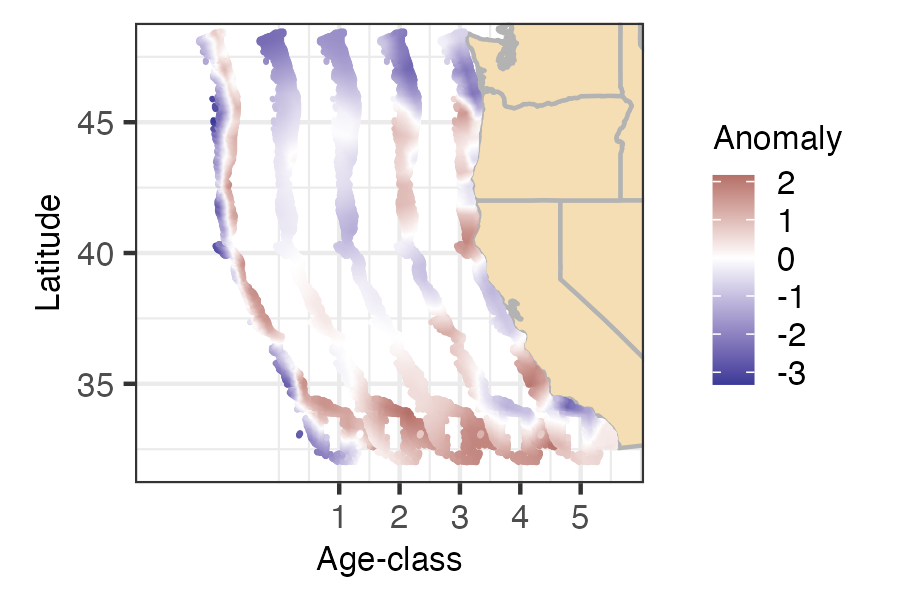
\includegraphics[width=3in,height=\textheight]{plots/hake_spatial_anomaly.png}

}

\caption{\label{fig-hake-spatial-anomaly}Estimated spatial anomalies for
Pacific hake ages 1 -- 5. These fields represent the average anomalies
across all years, 2003 -- 2023.}

\end{figure}%

\newpage

\begin{figure}

\centering{

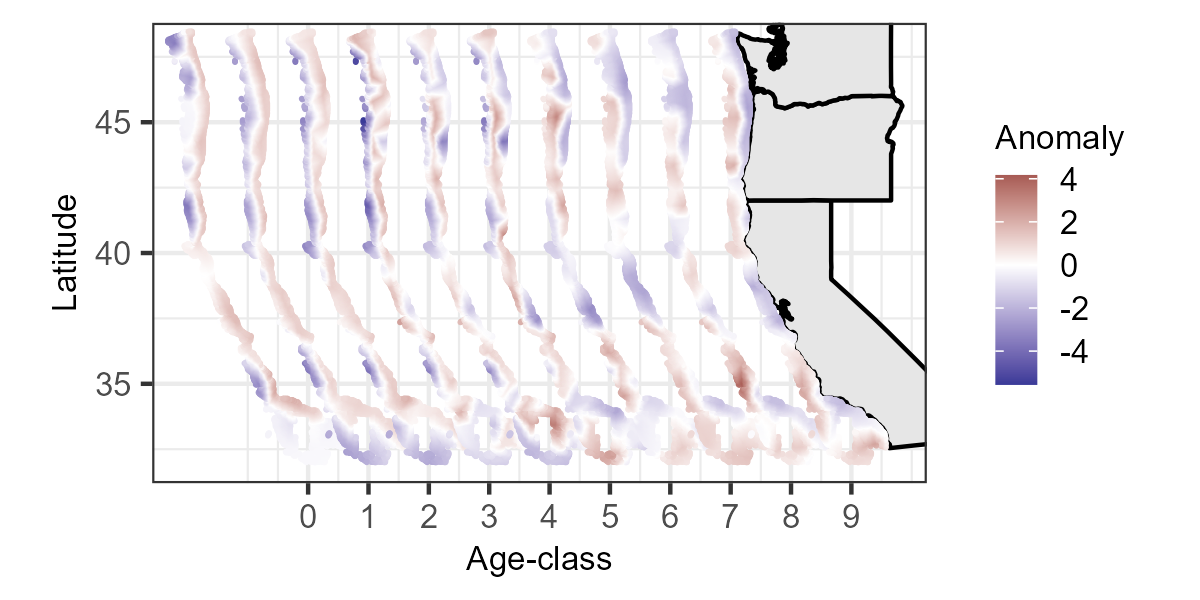
\includegraphics[width=4in,height=\textheight]{plots/sablefish-spatial-anomaly.png}

}

\caption{\label{fig-sablefish-spatial-anomaly}Estimated spatial
anomalies for sablefish ages 0 -- 9. These fields represent the average
anomalies across all years, 2003 -- 2023.}

\end{figure}%

\newpage

\begin{figure}

\centering{

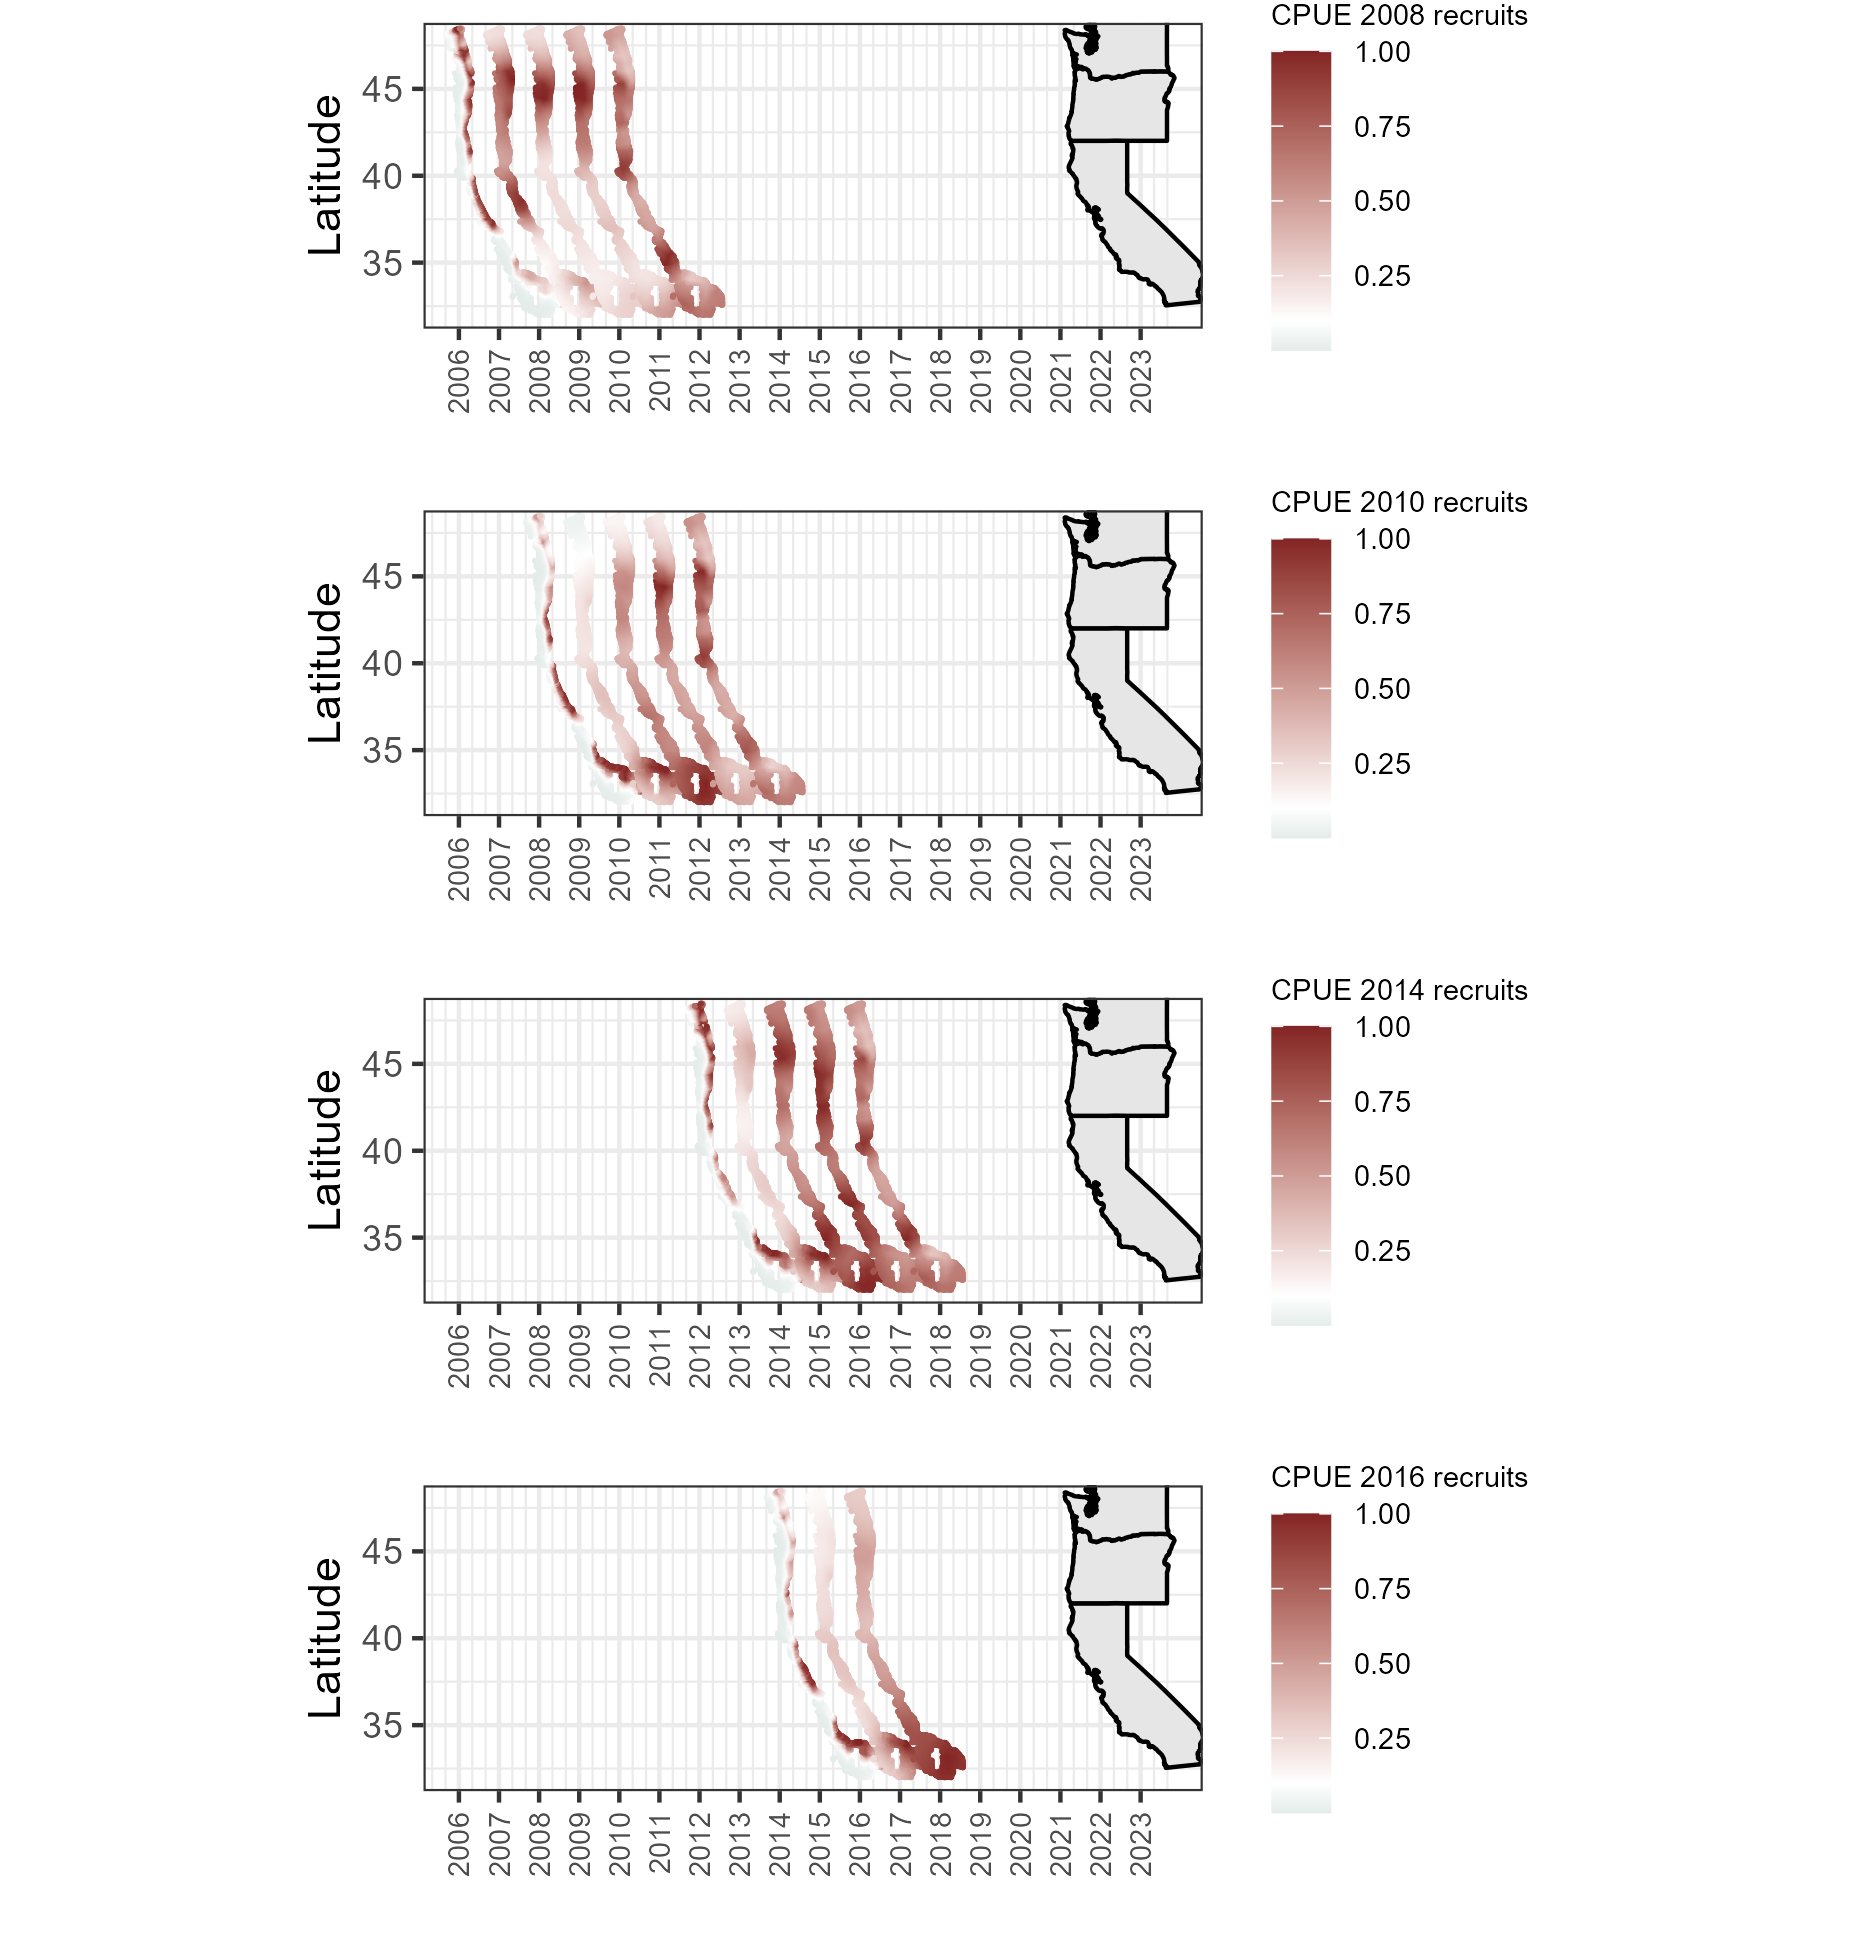
\includegraphics[width=6.2in,height=\textheight]{plots/Pacific hake-follow-age-class.png}

}

\caption{\label{fig-hake-spatial-composition}Estimated spatial catch per
unit effort (CPUE, kg per km2) for Pacific hake; rows represent strong
cohorts in our dataset (2008, 2010, 2014, 2016). CPUE is standardized to
1.0 across cohorts for visualization purposes. Full predictions for all
cohorts are in the Supplementary Information.}

\end{figure}%

\newpage

\begin{figure}

\centering{

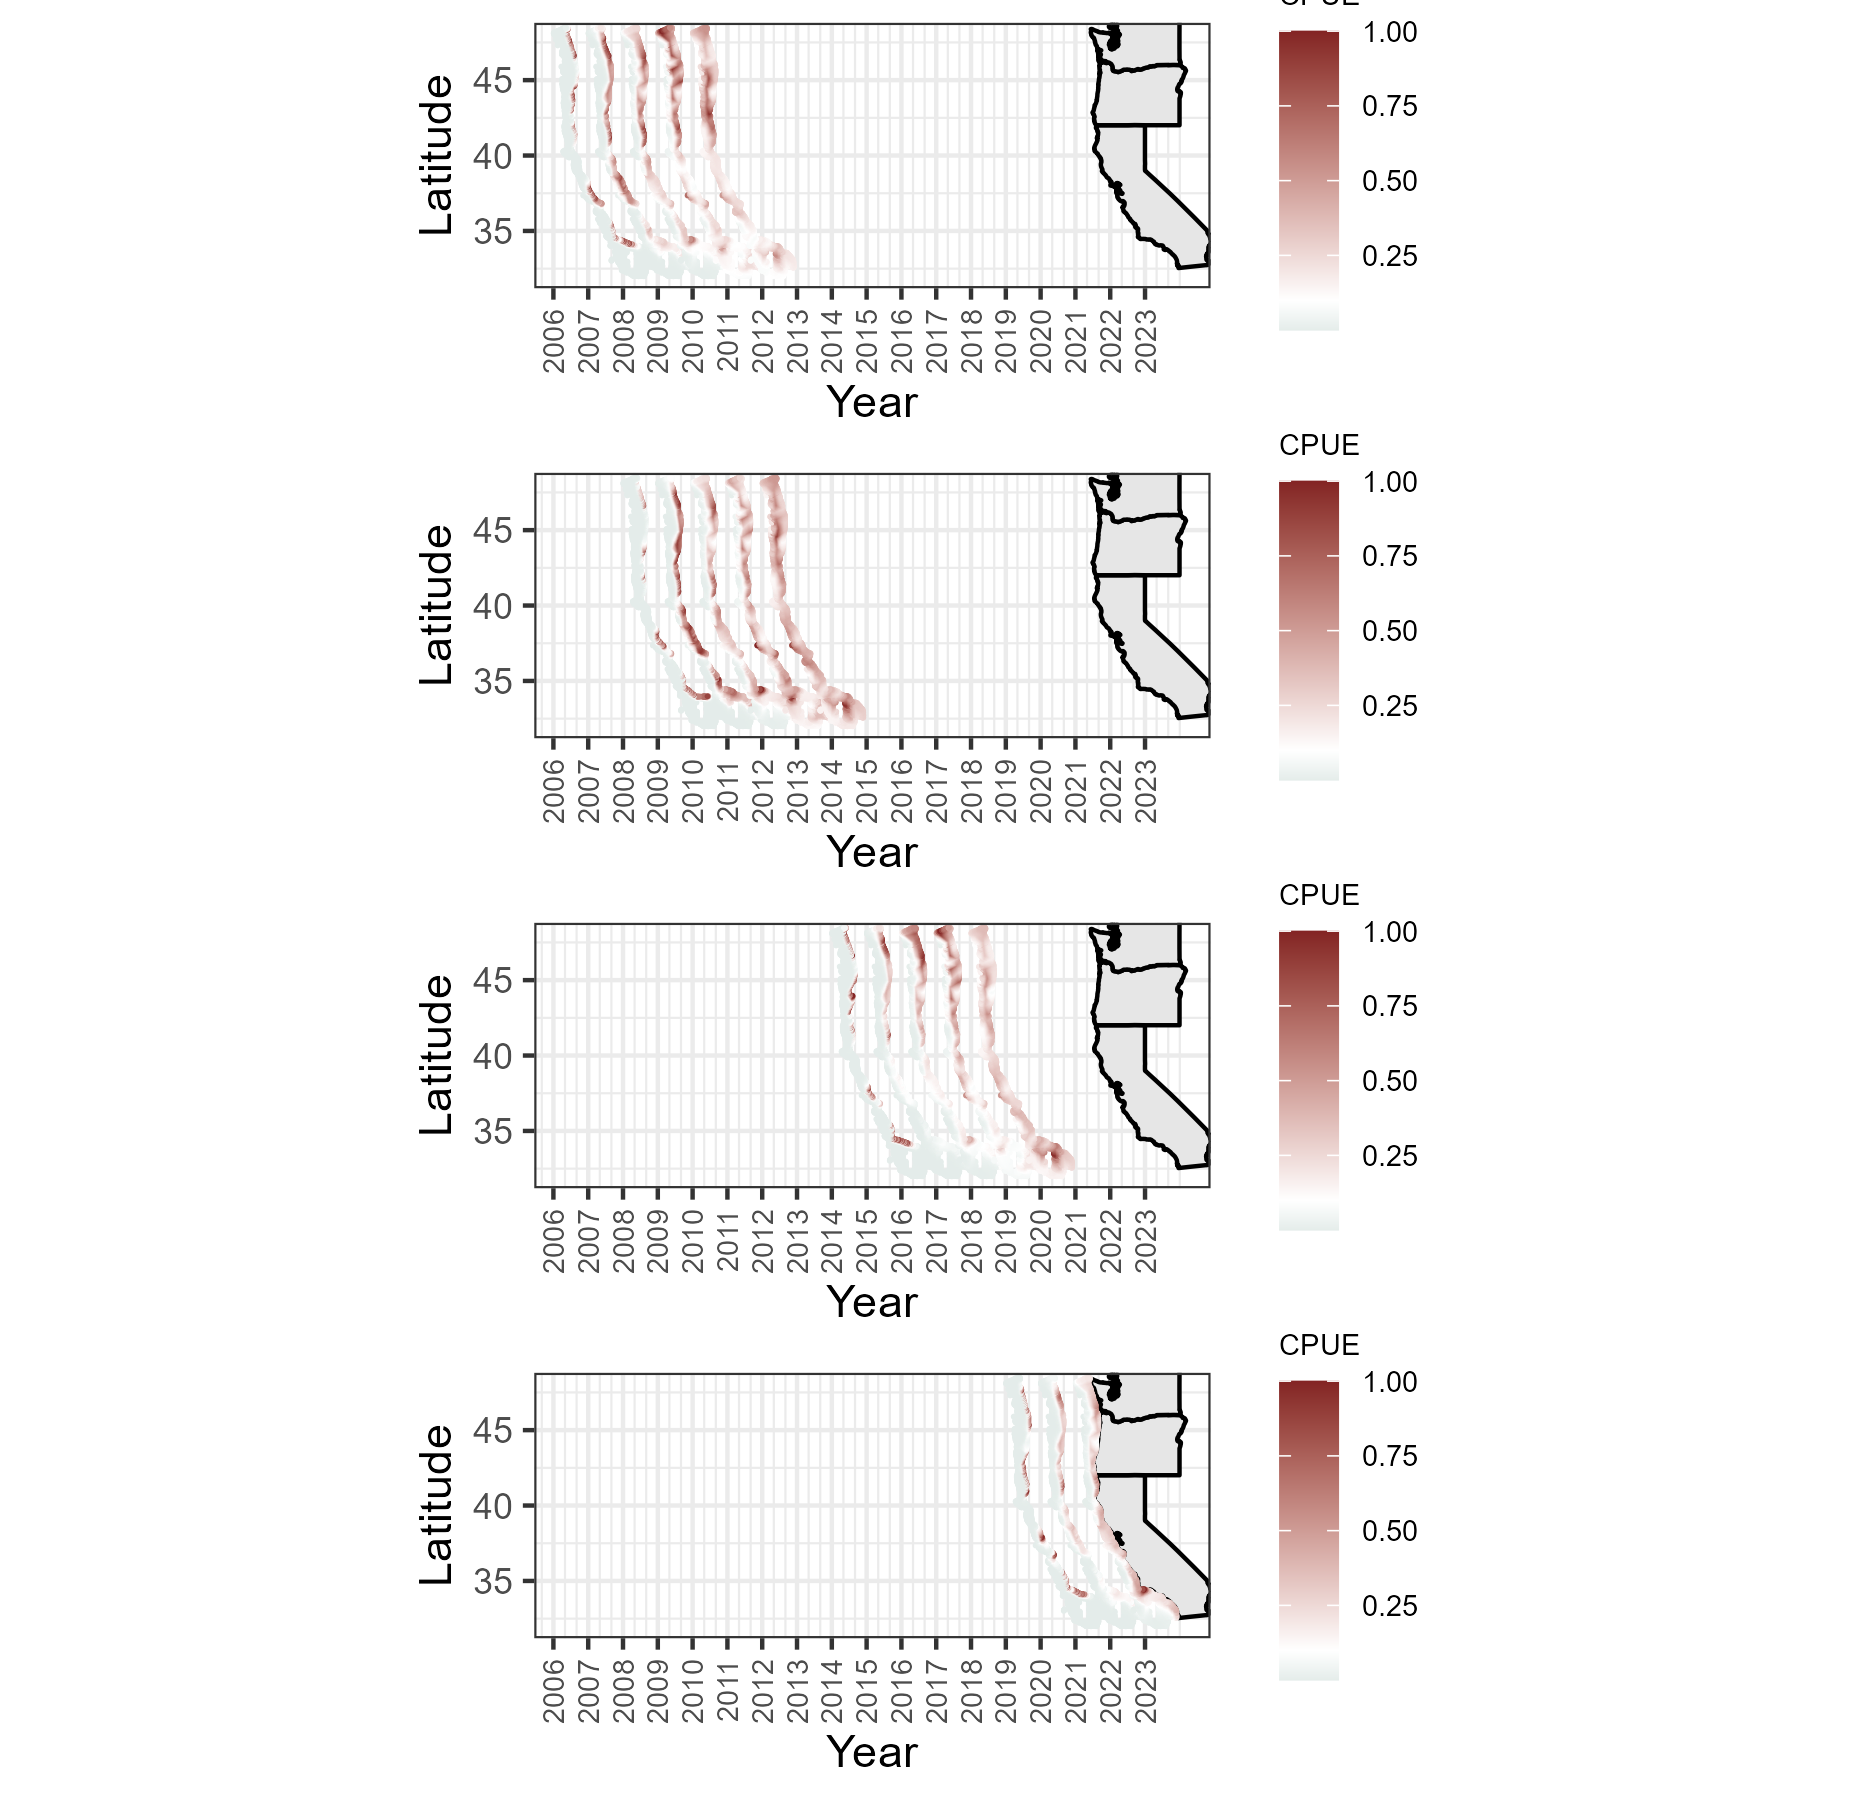
\includegraphics[width=6.2in,height=\textheight]{plots/sablefish-follow-age-class.png}

}

\caption{\label{fig-sablefish-spatial-composition}Estimated spatial
catch per unit effort (CPUE, kg per km2) for sablefish; each row
represents a strong cohorts in our dataset (2008, 2010, 2016, 2021).
CPUE is standardized to 1.0 across cohorts for visualization purposes.
Full predictions for all cohorts are in the Supplementary Information.}

\end{figure}%

\newpage

\begin{figure}

\centering{

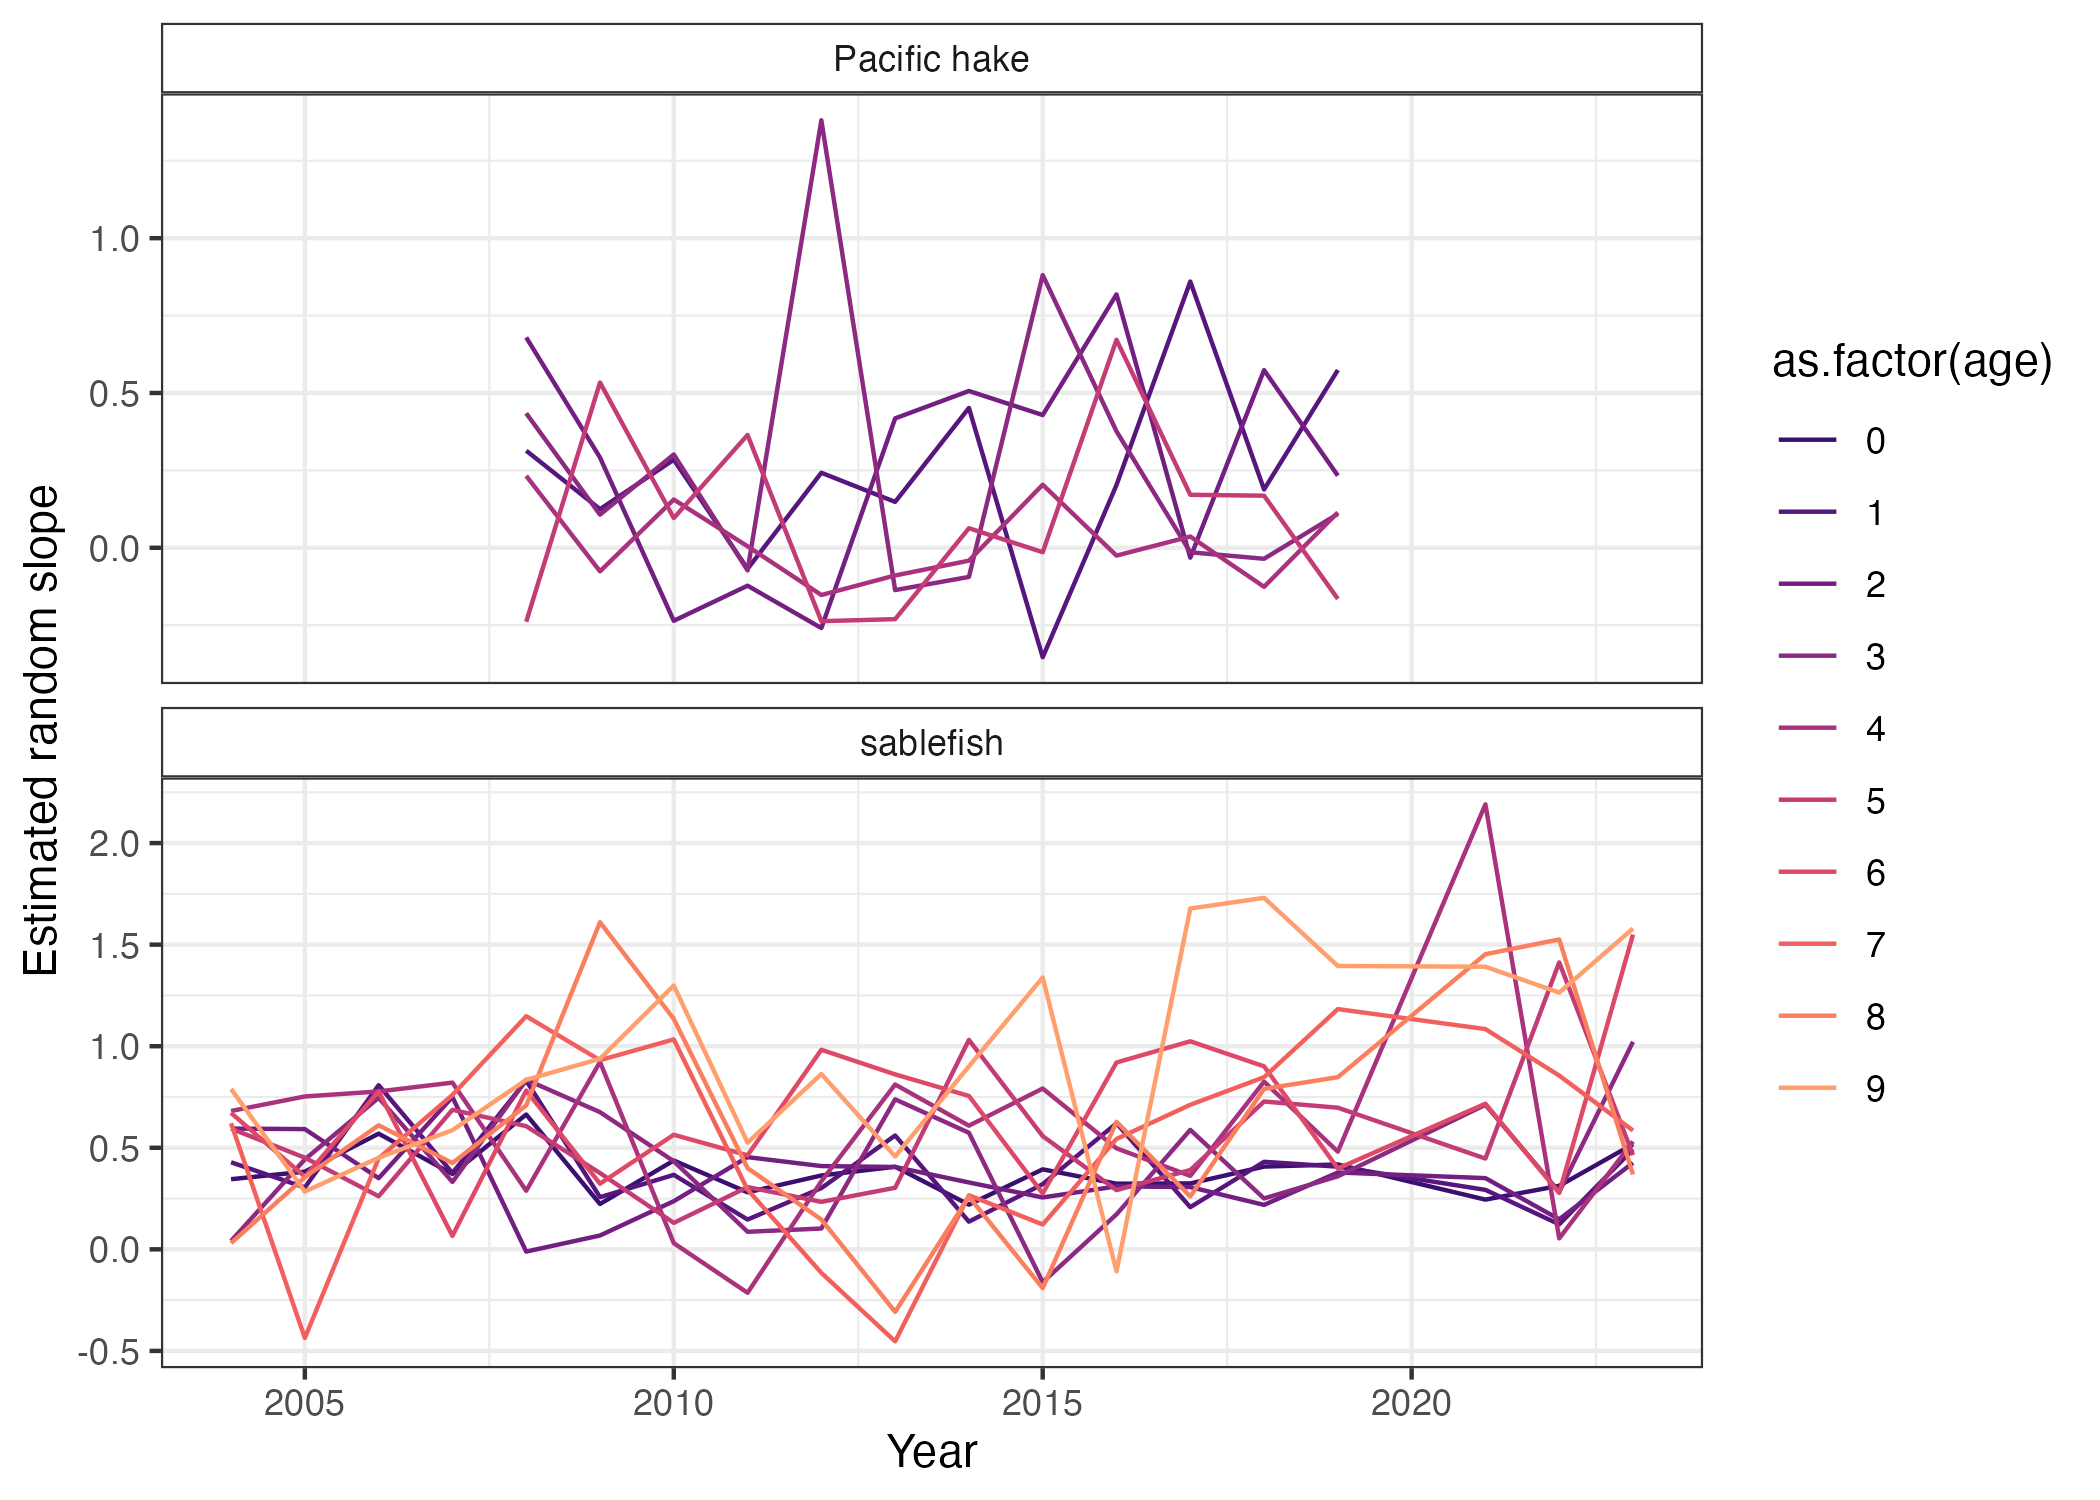
\includegraphics[width=3.5in,height=\textheight]{plots/glm_coefficients.png}

}

\caption{\label{fig-glm-coefficients}Estimated coefficients relating
predicted densities of age a fish in year t to observed numbers the
following year. The coefficients and 95\% confidence intervals (vertical
lines) are estimated in log space and presented here in normal space.}

\end{figure}%

\clearpage

\newpage

\begin{figure}

\centering{

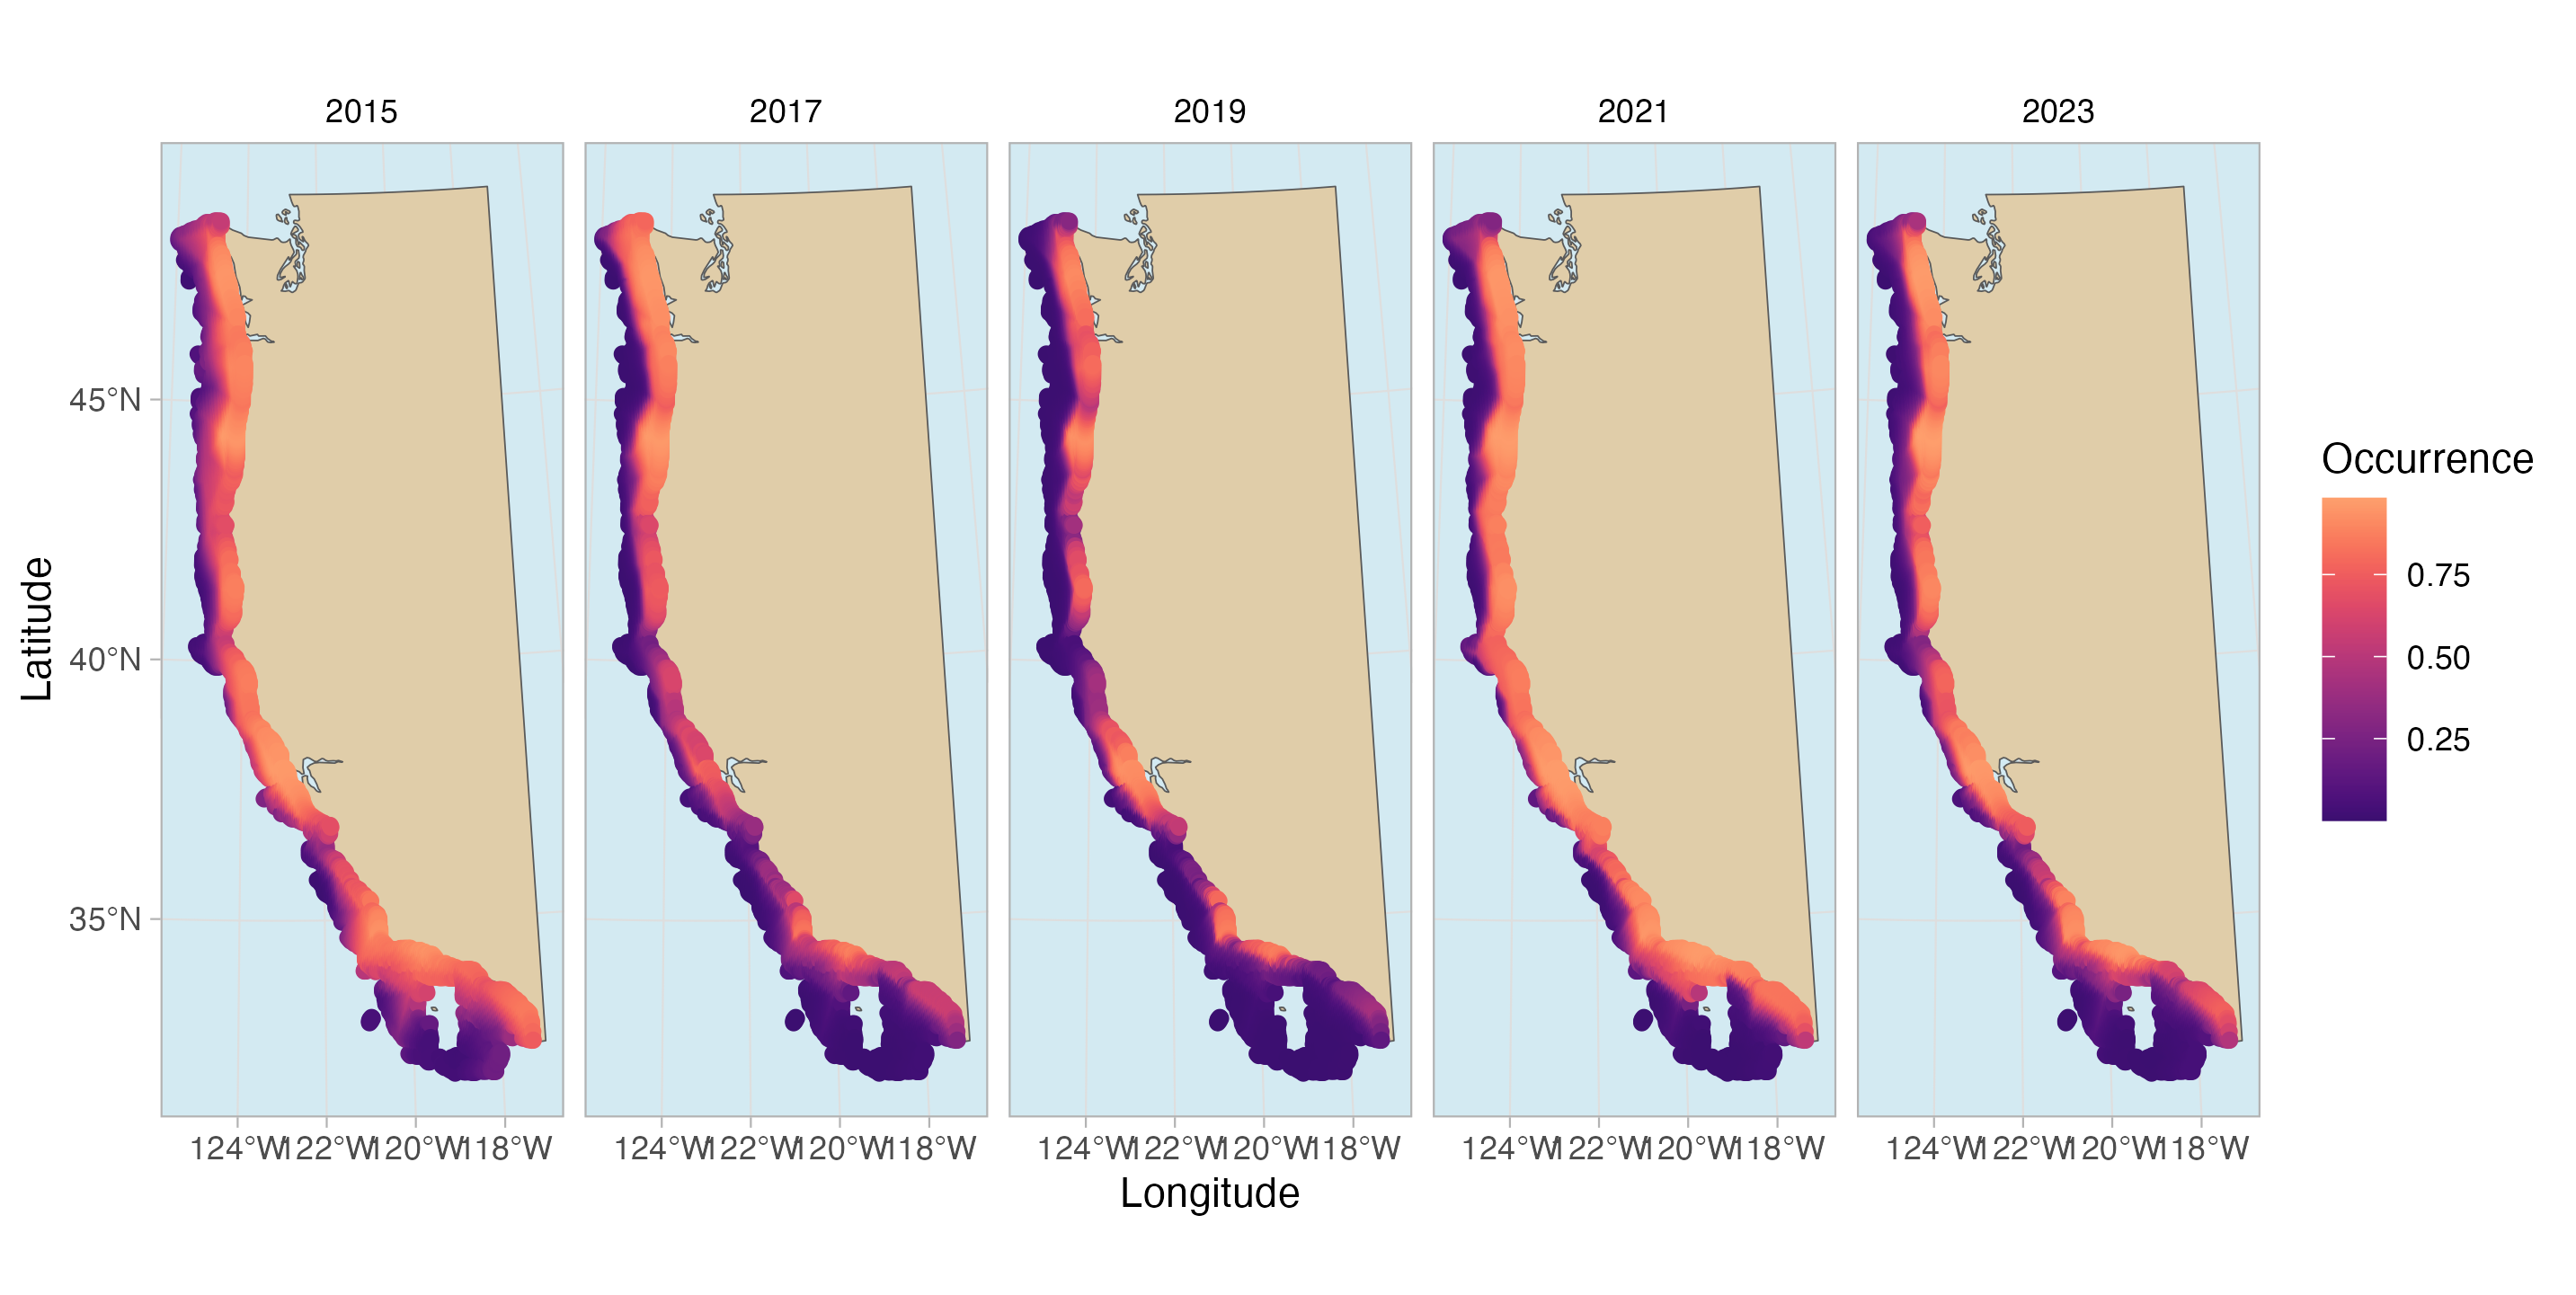
\includegraphics[width=5in,height=\textheight]{plots/sablefish_spatial_risk.png}

}

\caption{\label{fig-bycatch-risk}Estimated spatial catch per unit effort
(CPUE, kg per km2) for age-1 sablefish and port-level forecasts of age-1
CPUE within a radius of 232 km. In the upper plot CPUE is standardized
to 1.0 across cohorts for visualization purposes.}

\end{figure}%

\break
\clearpage

\section{Supplementary material}\label{supplementary-material}

\begin{figure}

\centering{

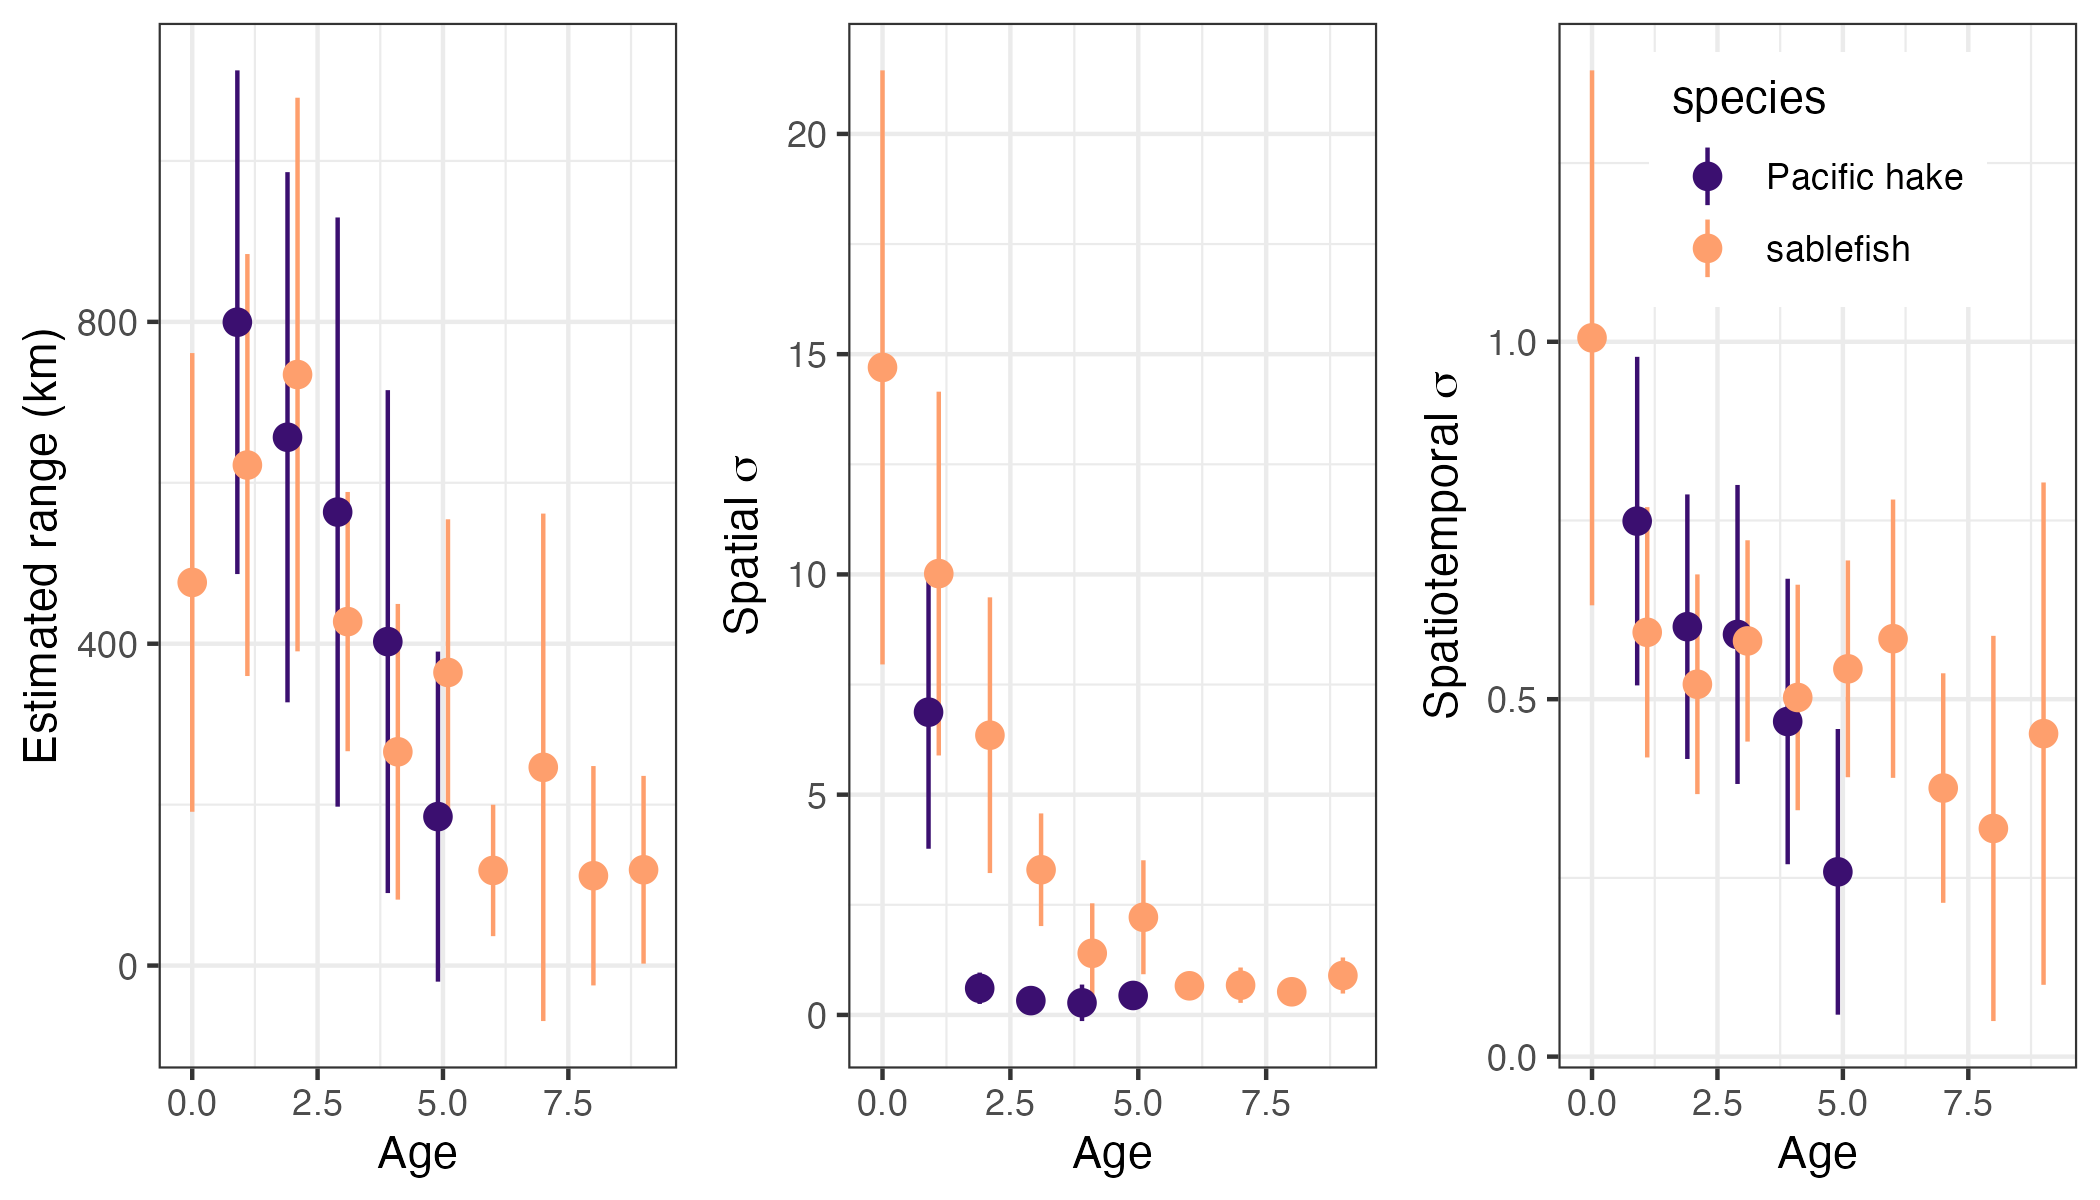
\includegraphics[width=5in,height=\textheight]{plots/spatial_parameters.png}

}

\caption{\label{fig-spatial-parameters}Estimated spatial parameters
(range, and spatial and spatiotemporal standard deviations). Points
represent mean estimates; lines represent 95\% confidence intervals}

\end{figure}%

\newpage

\begin{figure}

\centering{

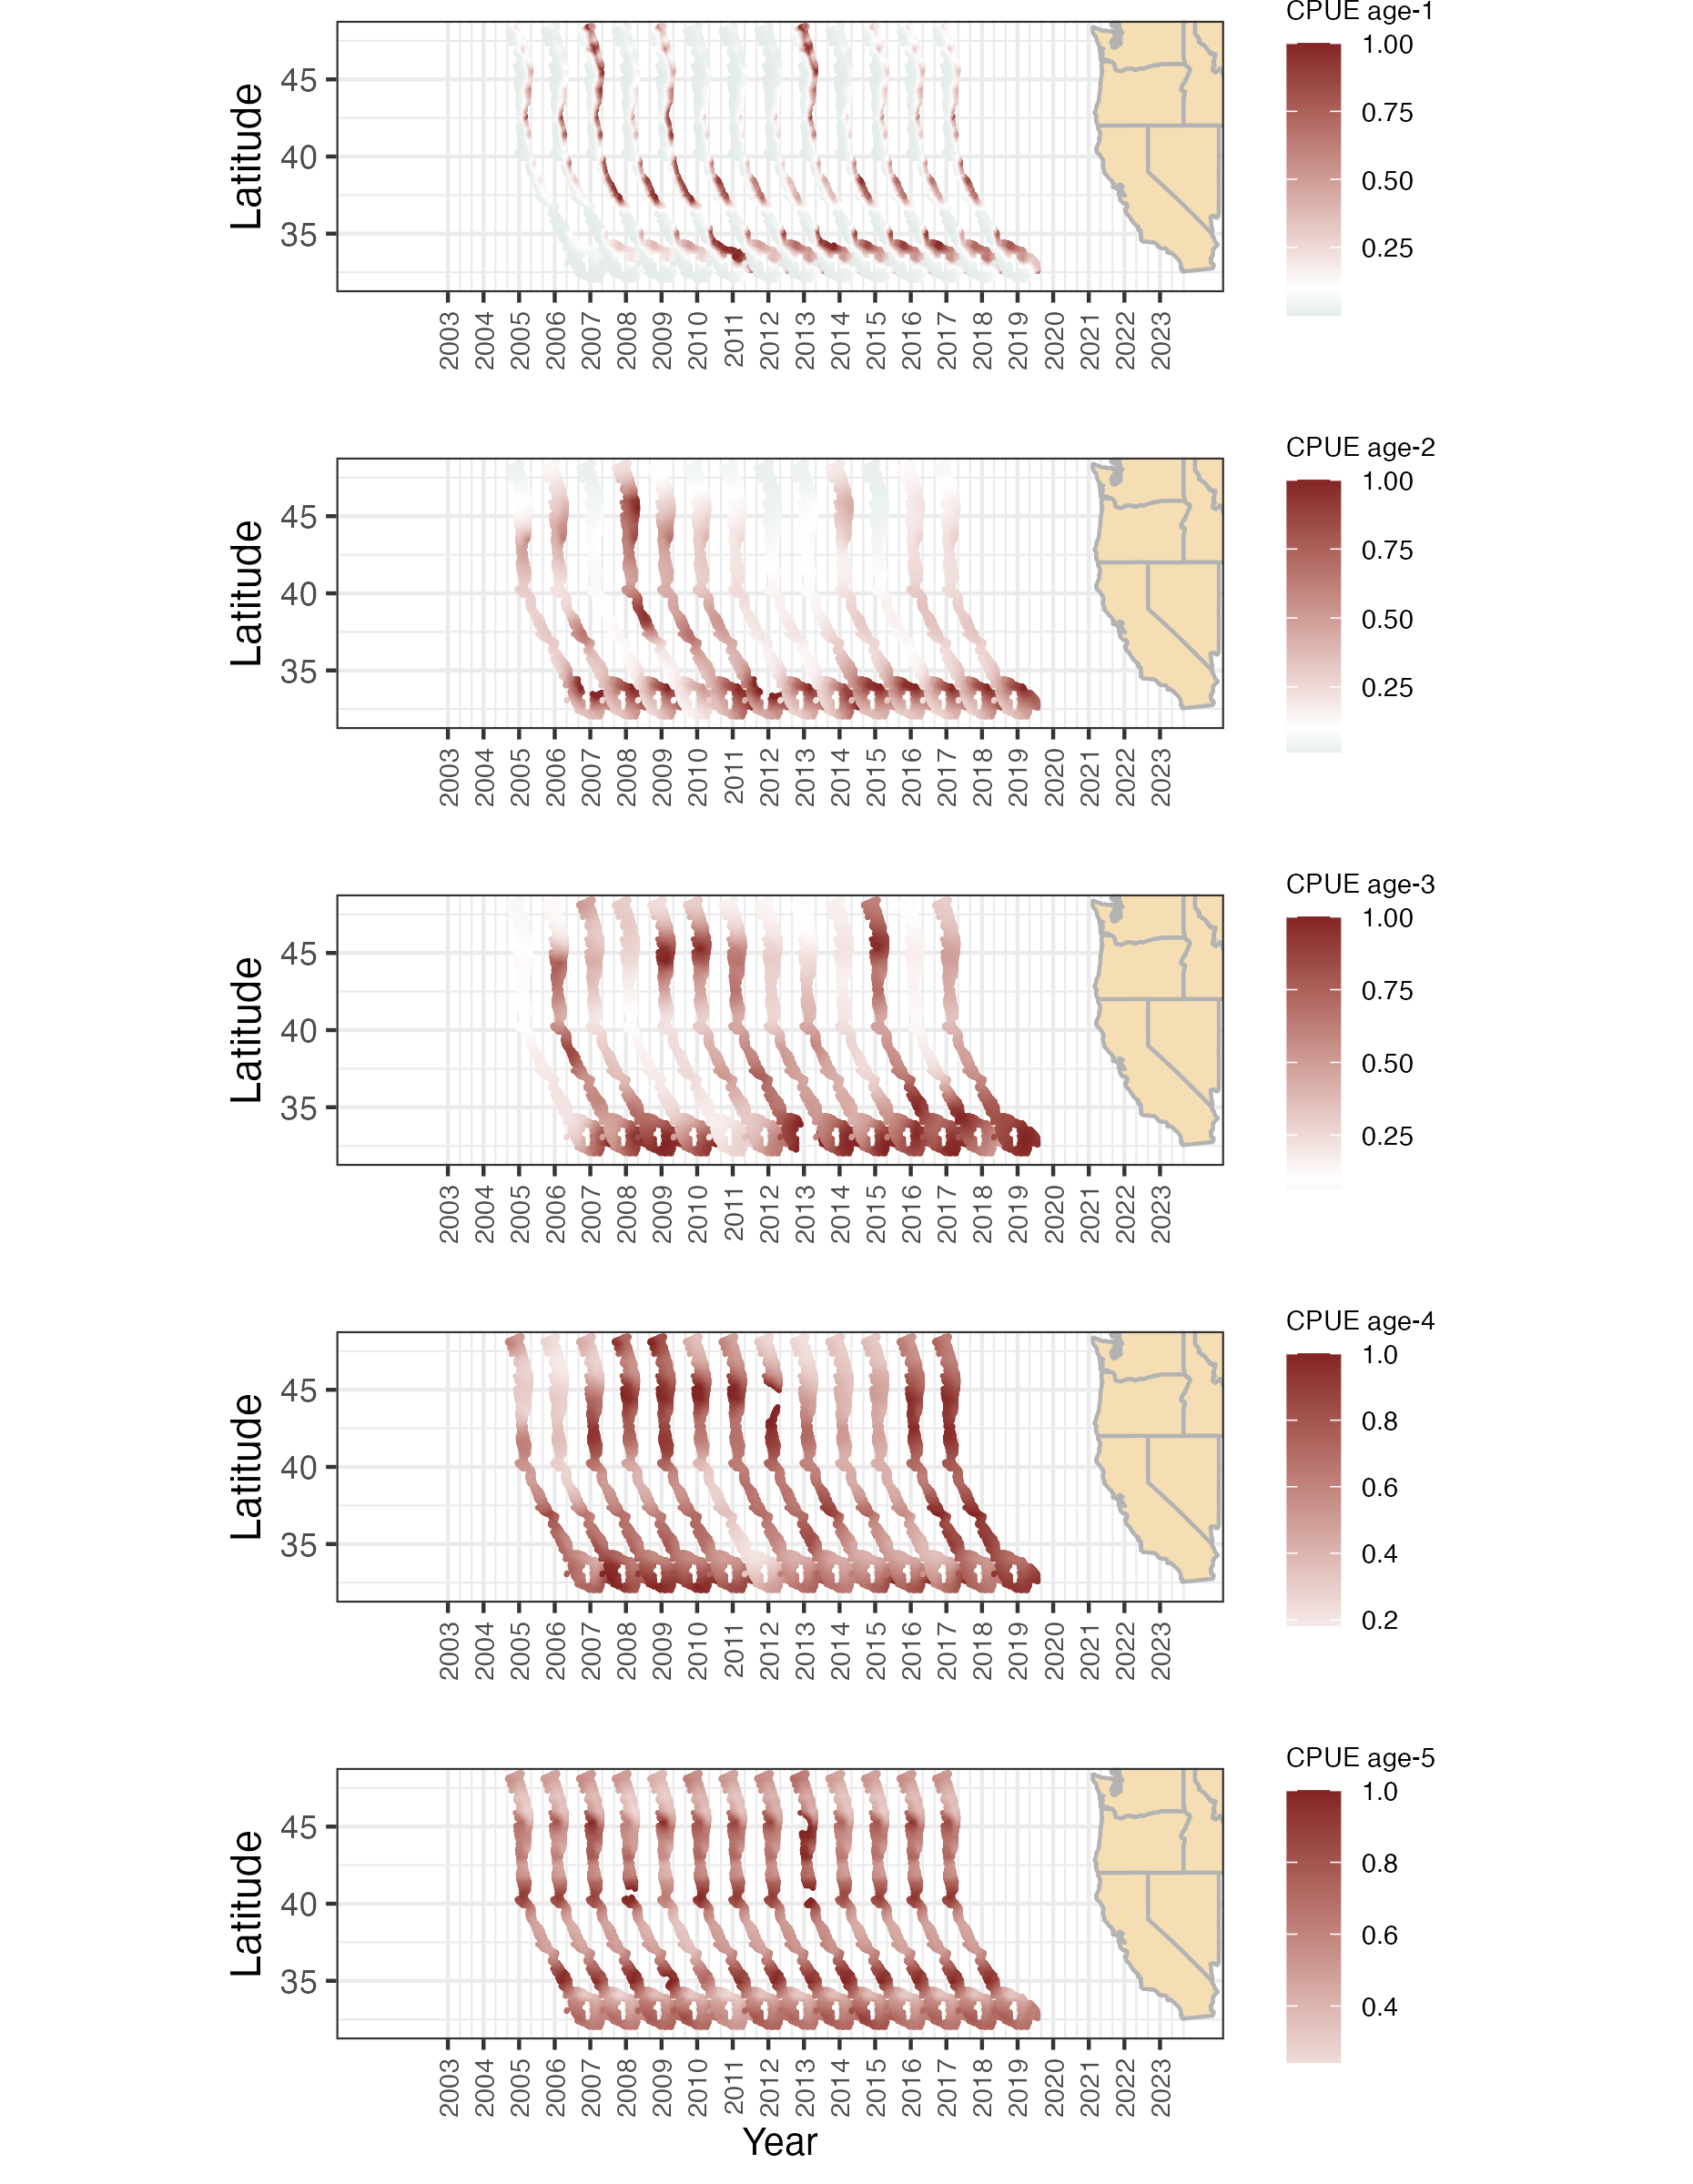
\includegraphics[width=6.2in,height=\textheight]{plots/Pacific hake-age-class-year.png}

}

\caption{\label{fig-hake-spatial-composition-all}Estimated spatial catch
per unit effort (CPUE, kg per km2) for Pacific hake; rows represent ages
(1-5). CPUE has been scaled for each cohort for visualization purposes.}

\end{figure}%

\newpage

\begin{figure}

\centering{

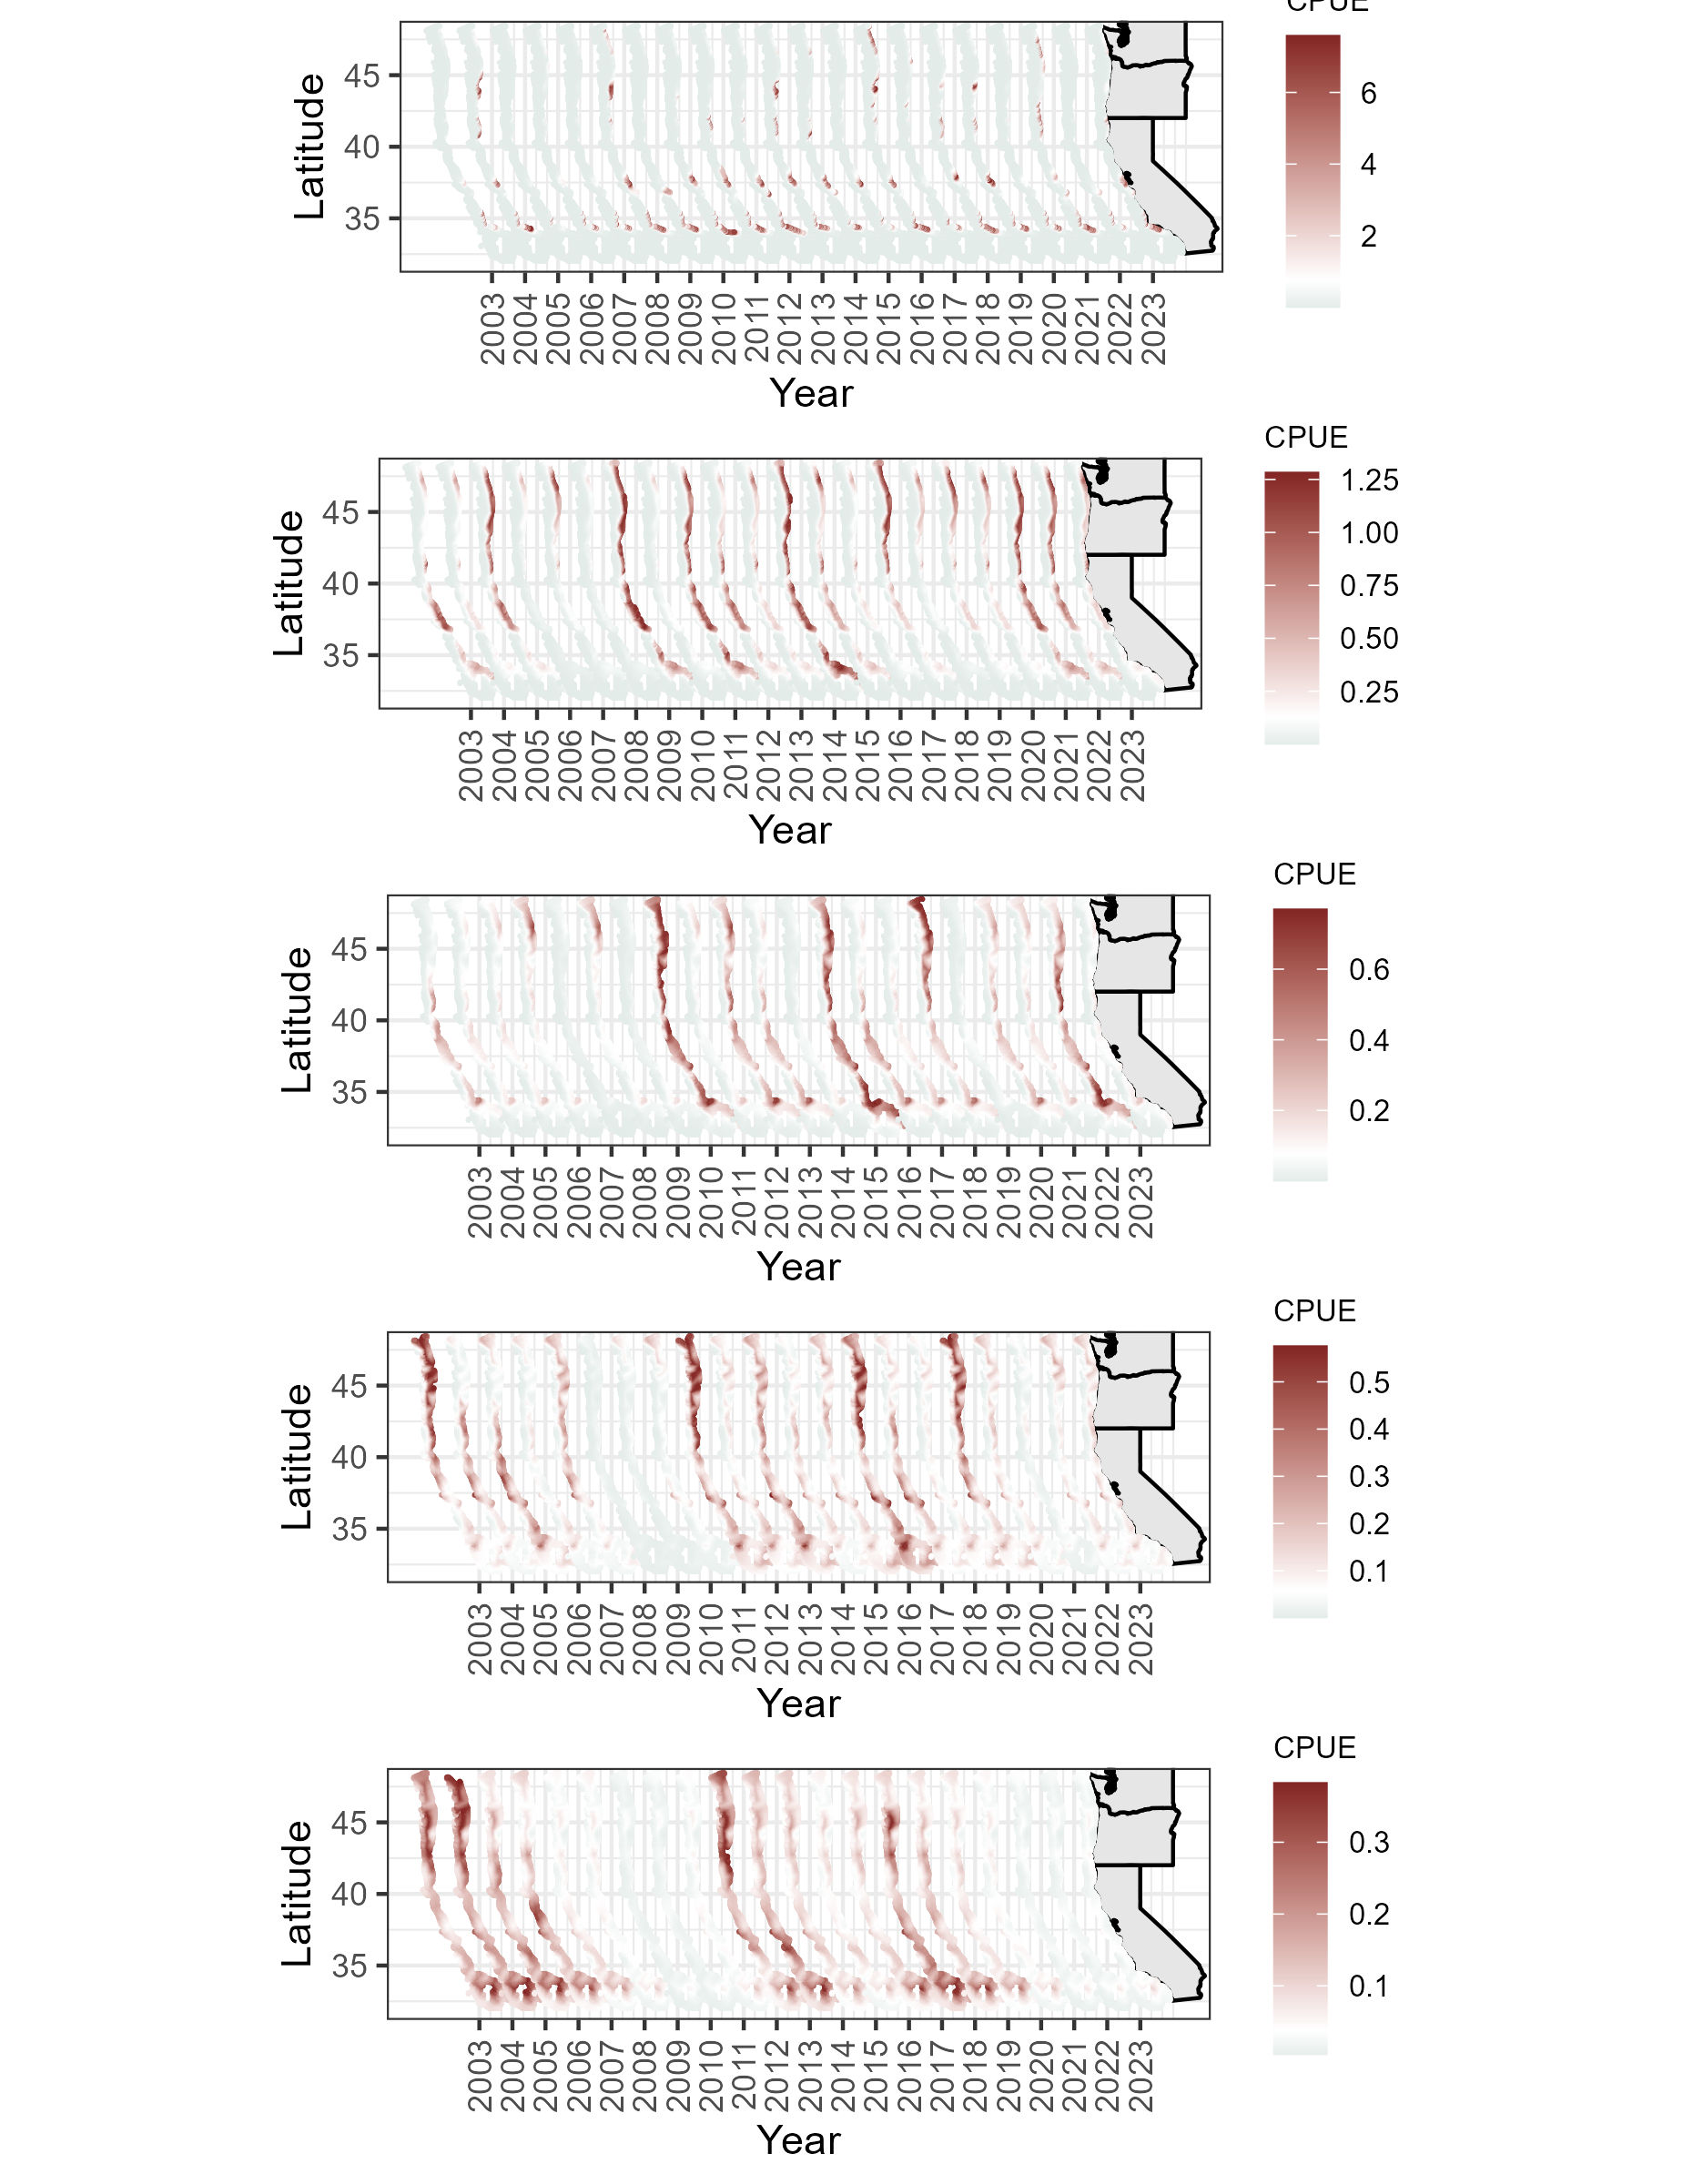
\includegraphics[width=6.2in,height=\textheight]{plots/sablefish-age-class-year.png}

}

\caption{\label{fig-sablefish-spatial-composition-all}Estimated spatial
catch per unit effort (CPUE, kg per km2) for sablefish; rows represent
ages (0-4). CPUE has been scaled for each cohort for visualization
purposes.}

\end{figure}%

\newpage

\begin{figure}

\centering{

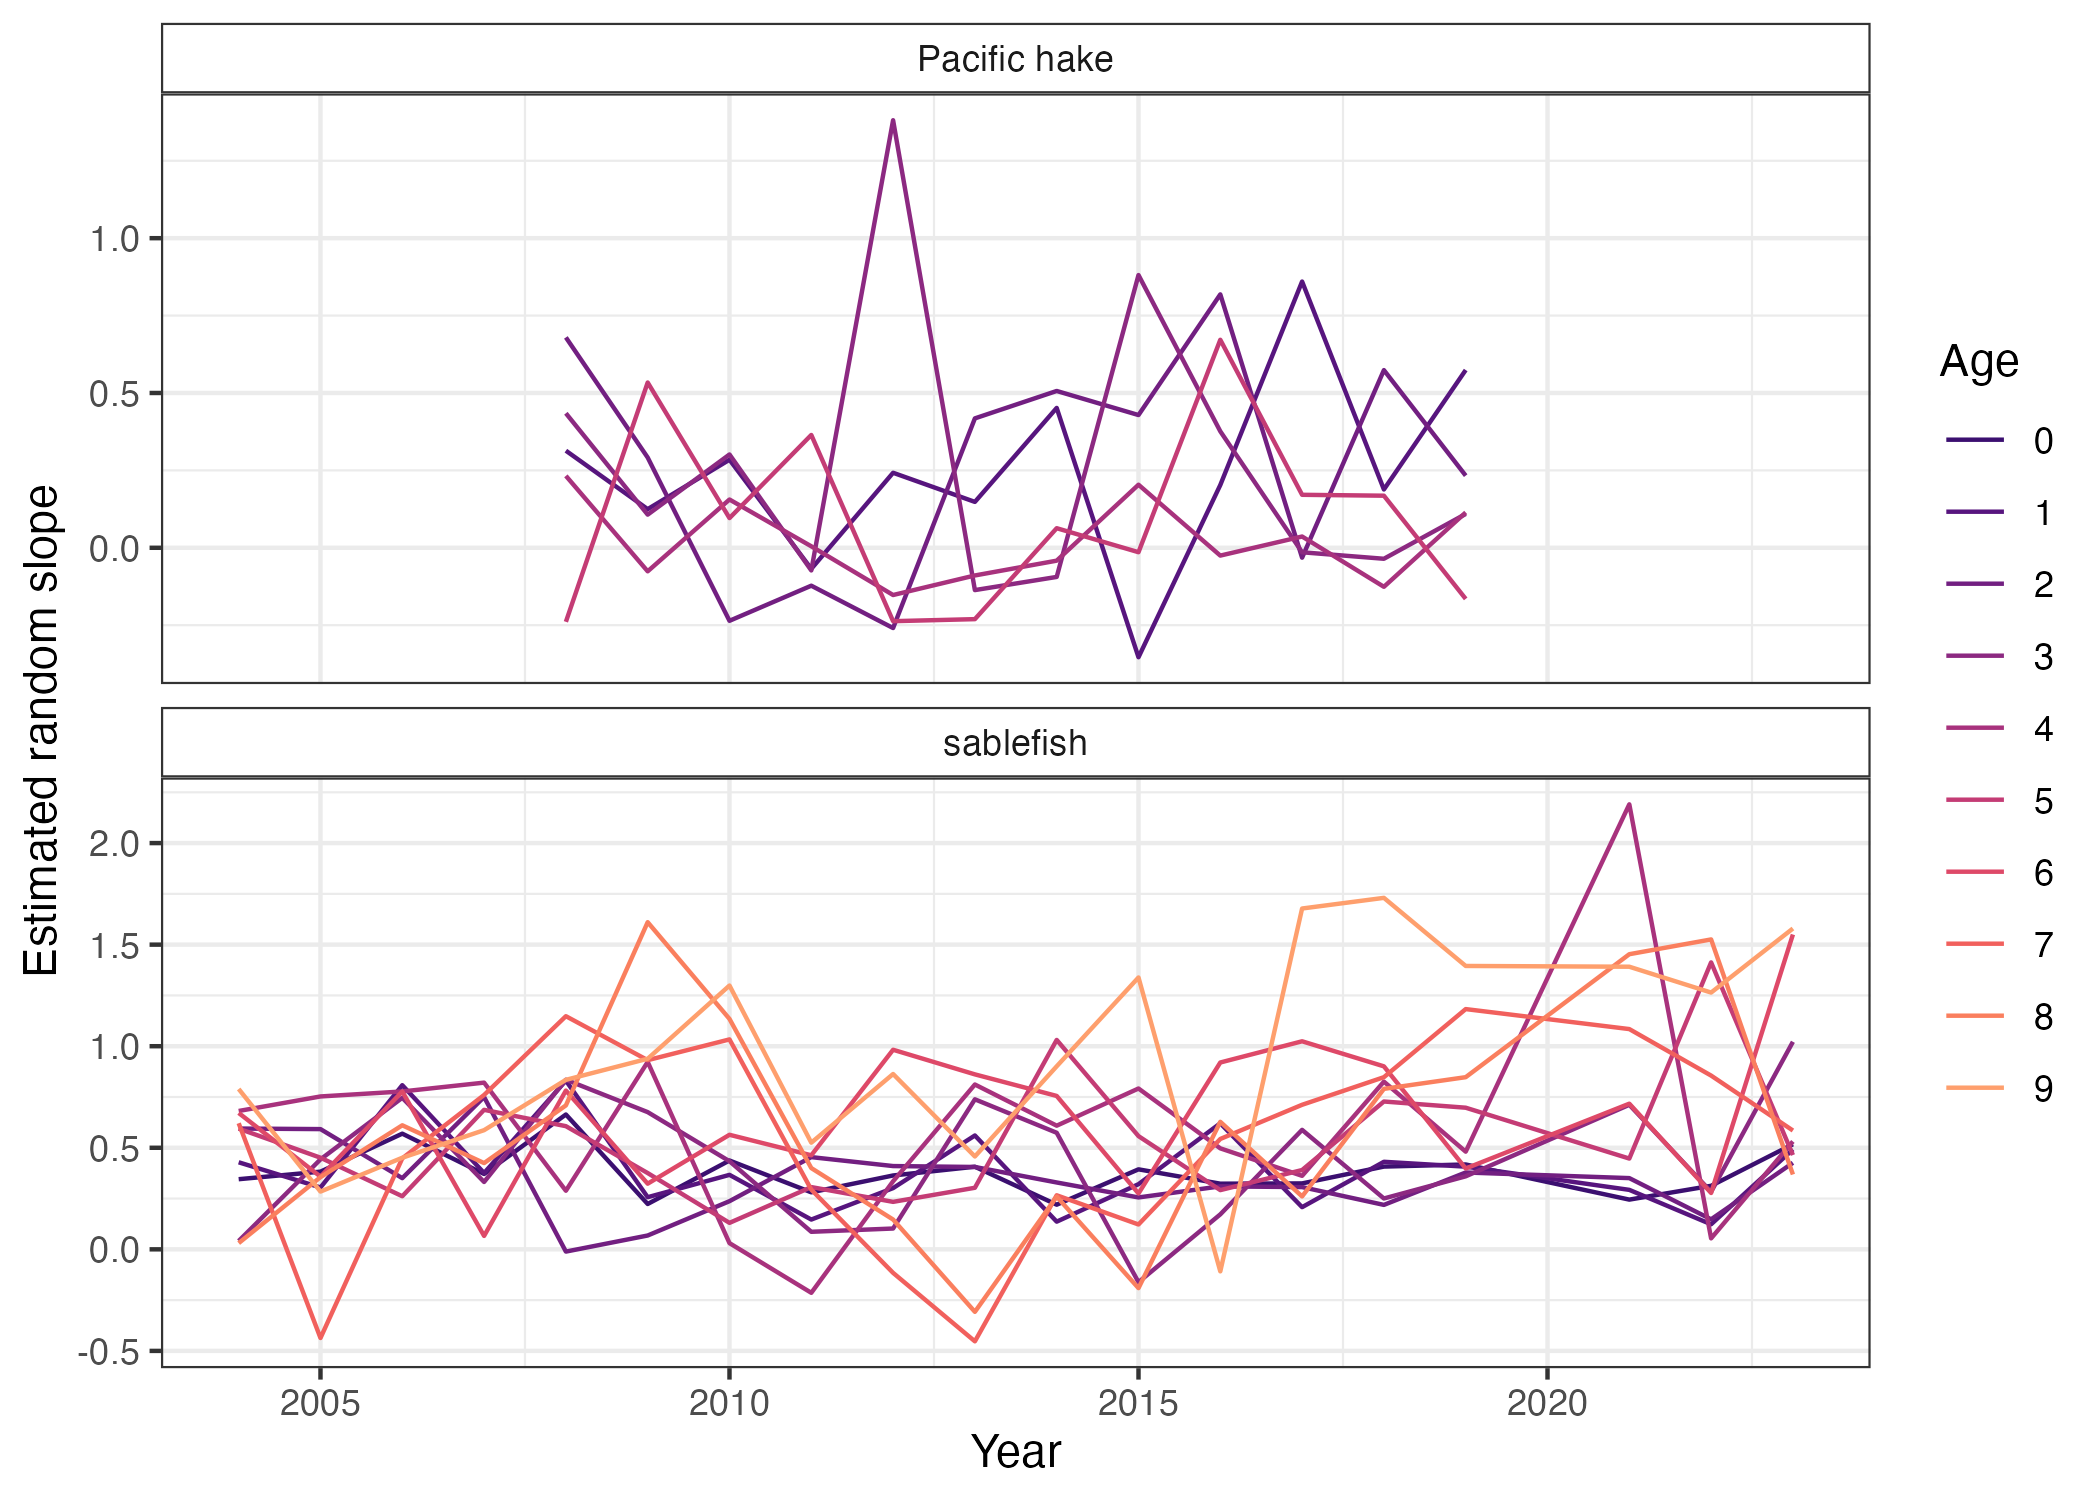
\includegraphics[width=7in,height=\textheight]{plots/glm_coefficients_time.png}

}

\caption{\label{fig-glm-coefficients-time}Time-varying coefficients
(with random effects in year) relating predicted densities of age a fish
in year t to observed numbers the following year.}

\end{figure}%



\end{document}
